\documentclass[11pt, onehalf, phd]{osudiss-2}
%\documentclass[ALICE,manyauthors]{ALICE_scientific_notes}
%
%\newcommand{\jpsi}{\rm J/$\psi$}
%\newcommand{\psip}{$\psi^\prime$}
%\newcommand{\jpsiDY}{\rm J/$\psi$\,/\,DY}
%\newcommand{\dd}{\mathrm{d}}
%\newcommand{\chic}{$\chi_{\rm c}$}
%\newcommand{\ezdc}{$E_{\rm ZDC}$}
%\newcommand{\red}{\textcolor{red}}
%\newcommand{\blue}{\textcolor{blue}}
%\newcommand{\slfrac}[2]{\left.#1\right/#2}
\usepackage{rotating}
\usepackage{comment} 
\usepackage{mhchem} % chemical index notation
%\usepackage{epsfig}
%\usepackage{epstopdf}
%\usepackage{graphicx}
% number the lines
\usepackage[modulo]{lineno,xcolor}
% Uncomment for running line numbers:
%\linenumbers
%\setlength\linenumbersep{5pt}
\renewcommand\linenumberfont{\normalfont\tiny\sffamily\color{gray}}
\providecommand{\abs}[1]{\left\lvert#1\right\rvert}

\newcommand\presentationsname{Presentations}
\newenvironment{preslist}
  {\vspace*{15pt}\begin{center}{{\typesetLevelThree\presentationsname}}
   \end{center}\vspace*{10pt}}
  {\vspace{\baselineskip}}
% Use with the |preslist| environment for presentation entries.
%    \begin{macrocode}
\newcommand\presitem[1]{\noindent #1 \par~~\par}

% clickable table of contents
\usepackage{color}   %May be necessary if you want to color links

\usepackage{hyperref}
\hypersetup{
    colorlinks=true, %set true if you want colored links
    linktoc=all,     %set to all if you want both sections and subsections linked
    linkcolor=blue,  %choose some color if you want links to stand out
   	%linkcolor={blue!50!black},
    %citecolor={green!50!black},
    %urlcolor={blue!80!black}
}

\usepackage{amsmath}
\usepackage{amsfonts}
\usepackage{amssymb}

% mark overfull hboxes
%\usepackage[width=5pt,
 %           height=0.5\baselineskip]{overcolored}

% Fix quotation marks
\usepackage [english]{babel}
\usepackage [autostyle, english = american]{csquotes}
\MakeOuterQuote{"}

% Center figures
\makeatletter
\g@addto@macro\@floatboxreset\centering
\makeatother

% Add backreferences
\usepackage[backend=biber,backref=true,sorting=none]{biblatex}
\addbibresource{bibfile.bib}
\DefineBibliographyStrings{english}{%
  backrefpage = {page},% originally "cited on page"
  backrefpages = {pages},% originally "cited on pages"
}

%
\begin{document}%
%%%%%%%%%%%%% ptdr definitions %%%%%%%%%%%%%%%%%%%%%
%
%%%%%%%%%%%%%%%  Title page %%%%%%%%%%%%%%%%%%%%%%%%
%
%\begin{titlepage}
%
%\EXPnumber{ALICE-INT-2012-xxx} %\EXPdate{31 October 2011}
%\PHdate{\today}
%
%
%%% Put your own title + short title here:
\title{Lambda femtoscopy in $\sqrt{s_{NN}}=2.76$ TeV Pb-Pb collisions at ALICE}
%\title{Lambda femtoscopy in $\sqrt{s_{NN}}=2.76$ TeV Pb-Pb collisions at ALICE}   % appears on right page headers
%
\author{Jai Salzwedel}
\advisorname{Professor Thomas Humanic}
\degree{Doctor of Philosophy} % Default value
\member{Professor Michael Lisa}
\member{Professor Yuri Kovchegov}
\member{Professor Fengyuan Yang}
\member{Professor Michael Bond}
\authordegrees{B.A. \&  M.S.}
\graduationyear{2017}
\unit{Graduate Program in Physics} % defaults to ``Graduate Program in Physics''

%\author{Email: jai.salzwedel@gmail.com}

%
\frontmatter
%\end{titlepage}
\begin{abstract}
Two-$\Lambda$ momentum correlation functions measured in Pb-Pb collisions at $\sqrt{s_{NN}}=2.76$ TeV by the ALICE collaboration are presented.  Results are shown for $\Lambda\Lambda$, $\bar{\Lambda}\bar{\Lambda}$ and $\Lambda\bar{\Lambda}$ pairs.


In this thesis, we will present lambda baryon femtoscopy measured by the ALICE collaboration in $\sqrt{s_{NN}}=2.76$ TeV Pb-Pb collision.
Correlation functions are shown in three centrality ranges for $\Lambda\bar{\Lambda}$ and two for the combined $\Lambda\Lambda\oplus\bar{\Lambda}\bar{\Lambda}$ results.


The standard femtoscopic fitting process has been expanded to account for the correlated effects of particles that decay into $\Lambda$. % Expand this
These are effects may be significant; it is estimated that only a quarter of pairs contain two primary $\Lambda$.
The rest contain one or two secondary $\Lambda$.
We have estimated the $\lambda$ parameters that describe the relative contribution of each residual correlation, and they are included in a table.
This technique has been used in the past to perform measurements of $\mathrm{p}\bar{\Lambda}$ and $\bar{\mathrm{p}}\bar{\mathrm{p}}$ scattering parameters.



Fit results have been found for femtoscopic radii of the pairs, with the 

, as well as for the complex scattering lengths $f_0$ and the effective range of interaction, the s-wave scattering parameters.

This approach may have applicability for measuring the poorly known interactions of other pairs, such as $\Lambda\Xi^-$, $\Lambda K^-$, or $Xi^-K^-$.
\end{abstract}

%\dedication{To my loving family (yes, even the ones that meow at me in the middle of the night)}
%\begin{acknowledgments}

I would like to thank my advisor, Tom Humanic, for all of his support these many years, and Mike Lisa as well.
I appreciate them for their mentorship and for guiding my research, challenging my assumptions, and sharing decades of experience with me.
I owe many thanks to them and to The Ohio State University physics department for an excellent education and the opportunity to travel the world in the name of science. 
Thanks to Kris Dunlap; she is the glue that holds the department together, and every student owes her a debt for the often unseen service and support she provides.

I am also indebted to the current and former students in the OSU Experimental Nuclear Physics group, and to the theorists across the hall. 
They were there at the start to mentor me as I was trying to wrap my head around this field, and they've been alongside me ever since.
Whether I needed a physicist's intuition, a programming tutor, a math consultant, or just someone to listen as I babbled in front of a white board, they were there.

I want to thank the ALICE Collaboration for allowing me to participate in cutting-edge science.
I'm particularly thankful to the AliFemto research group, within which I have found mentors, colleagues, and friends.

Thanks to Willamette University and University Prep for nurturing my curiosity and appreciation of science.
I would never have ended up here if not for the strong role models I had each step of the way.

I must thank my friends and family---my parents in particular---for years of love, support, and encouragement.

Finally, I thank my loving wife Amy for everything. Just everything.

% Mike
% osu group (call out John?)
% alice collaboration
% femtoscopy group
% Amy
% family
% friends


\end{acknowledgments}

\begin{Vita}
\dateitem{September 20, 1985}{Born---Seattle, WA}
\dateitem{May 2004}{Diploma, University Preparatory Academy, Seattle, Washington}
\dateitem{May 2008}{B.A. in Physics and Philosophy, Willamette University, Salem, Oregon}
\dateitem{August 2012}{M.S. in Physics, The Ohio State University, Columbus, Ohio}


% Insert other relevant items here (GTA, etc.)
%
\begin{publist}
%\pubitem{``Kinetic effects of solid density perturbations produced by intense laser pulses incident on reduced mass targets in {LSP}'' F. W. King, C. Orban, D. W. Schumacher, \textit{In internal review}.}
%\pubitem{``Modeling the effects of front-surface structures on target normal sheath acceleration using handoffs between multiple simulations" M. M. McMahon, F. W. King, D. W. Schumacher, \emph{et al.} \textit{In internal review}.}
%\pubitem{``Order and chaos in the rotation and revolution of a line segment and a point mass'' J. F. Lindner, J. Lynn, F. W. King, A. Logue, \textit{Phys. Rev. E} \textbf{81}, 036208 (2010).}

%\documentclass{article}
%\usepackage{textcomp} % text version of symbols in TS1, e.g. \textrightarrow{}
%\usepackage{amstext} % proper support of frequently used \text{} command
%To use pdflatex, uncomment these lines, as well as the \href lines
%in each entry
%\usepackage[pdftex,
%       colorlinks=true,
%       urlcolor=blue,       % \href{...}{...} external (URL)
%       filecolor=green,     % \href{...} local file
%       linkcolor=red,       % \ref{...} and \pageref{...}
%       pdftitle={Papers by AUTHOR},
%       pdfauthor={Your Name},
%       pdfsubject={Just a test},
%       pdfkeywords={test testing testable},
%       pagebackref,
%       pdfpagemode=None,
%        bookmarksopen=true]{hyperref}
%usepackage{arial}
%\renewcommand{\familydefault}{\sfdefault} % San serif
%\renewcommand{\labelenumii}{\arabic{enumi}.\arabic{enumii}}
%
%\pagestyle{empty}
%\oddsidemargin 0.0in
%\textwidth 6.5in
%\topmargin -0.75in
%\textheight 9.5in

%\begin{publist}
\begin{enumerate}
%%   LIST OF PAPERS
%%   Please comment out anything between here and the
%%   first \item
%%   Please send any updates or corrections to the list to
%%   admin@inspirehep.net
%\cite{Alice:2016wka}
\item%{Alice:2016wka}
{\bf ``W and Z boson production in p-Pb collisions at $\sqrt{s_{\rm NN}}$ = 5.02 TeV''}
  \\{}J.~Adam {\it et al.} [ALICE Collaboration].
  \\{}arXiv:1611.03002 [nucl-ex]
  \\{}CERN-EP-2016-278
%(Nov 9, 2016)
\href{http://inspirehep.net/record/1496634}{HEP entry}

%\cite{Adam:2016ilk}
\item%{Adam:2016ilk}
{\bf ``Determination of the event collision time with the ALICE detector at the LHC''}
  \\{}J.~Adam {\it et al.} [ALICE Collaboration].
  \\{}arXiv:1610.03055 [physics.ins-det]
  \\{}CERN-EP-2016-253
%(Oct 8, 2016)
\href{http://inspirehep.net/record/1491202}{HEP entry}

%\cite{Adam:2016khe}
\item%{Adam:2016khe}
{\bf ``Measurement of the production of high-$p_{\rm T}$ electrons from heavy-flavour hadron decays in Pb-Pb collisions at $\mathbf{\sqrt{\it s_{\rm{NN}}}}$ = 2.76 TeV''}
  \\{}J.~Adam {\it et al.} [ALICE Collaboration].
  \\{}arXiv:1609.07104 [nucl-ex]
  \\{}CERN-EP-2016-235
%(Sep 22, 2016)
\href{http://inspirehep.net/record/1487727}{HEP entry}

%\cite{Adam:2016ckp}
\item%{Adam:2016ckp}
{\bf ``Evolution of the longitudinal and azimuthal structure of the near-side jet peak in Pb-Pb collisions at $\sqrt{s_{\rm NN}} = 2.76$ TeV''}
  \\{}J.~Adam {\it et al.} [ALICE Collaboration].
  \\{}arXiv:1609.06667 [nucl-ex]
  \\{}CERN-EP-2016-228
%(Sep 21, 2016)
\href{http://inspirehep.net/record/1487546}{HEP entry}

%\cite{Adam:2016tsv}
\item%{Adam:2016tsv}
{\bf ``Anomalous evolution of the near-side jet peak shape in Pb-Pb collisions at $\sqrt{s_{\rm NN}}$ = 2.76 TeV''}
  \\{}J.~Adam {\it et al.} [ALICE Collaboration].
  \\{}arXiv:1609.06643 [nucl-ex]
  \\{}CERN-EP-2016-229
%(Sep 21, 2016)
\href{http://inspirehep.net/record/1487545}{HEP entry}

%\cite{Adam:2016wyz}
\item%{Adam:2016wyz}
{\bf ``Measurement of electrons from beauty-hadron decays in p-Pb collisions at $\mathbf{\sqrt{s_{\rm NN}}=5.02}$ TeV and Pb-Pb collisions at $\mathbf{\sqrt{s_{\rm NN}}=2.76}$ TeV''}
  \\{}J.~Adam {\it et al.} [ALICE Collaboration].
  \\{}arXiv:1609.03898 [nucl-ex]
  \\{}CERN-EP-2016-222
%(Sep 13, 2016)
\href{http://inspirehep.net/record/1486391}{HEP entry}

%\cite{Adam:2016xbp}
\item%{Adam:2016xbp}
{\bf ``Jet-like correlations with neutral pion triggers in pp and central Pb–Pb collisions at 2.76 TeV''}
  \\{}J.~Adam {\it et al.} [ALICE Collaboration].
  \\{}arXiv:1608.07201 [nucl-ex]
  \\{}DOI:10.1016/j.physletb.2016.10.048
  \\{}Phys.\ Lett.\ B {\bf 763}, 238 (2016)
  \\{}CERN-EP-2016-195
%(Aug 25, 2016)
\href{http://inspirehep.net/record/1483164}{HEP entry}
%2 citations counted in INSPIRE as of 01 Dec 2016
%\cite{Adam:2016rdg}
\item%{Adam:2016rdg}
{\bf ``J/$\psi$ suppression at forward rapidity in Pb-Pb collisions at $\mathbf{\sqrt{s_{{\rm NN}}} = 5.02}$ TeV''}
  \\{}J.~Adam {\it et al.} [ALICE Collaboration].
  \\{}arXiv:1606.08197 [nucl-ex]
  \\{}CERN-EP-2016-162
%(Jun 27, 2016)
\href{http://inspirehep.net/record/1472319}{HEP entry}
%12 citations counted in INSPIRE as of 01 Dec 2016
%\cite{Adam:2016emw}
\item%{Adam:2016emw}
{\bf ``Multiplicity-dependent enhancement of strange and multi-strange hadron production in proton-proton collisions at $\sqrt{s} = 7$ TeV''}
  \\{}J.~Adam {\it et al.} [ALICE Collaboration].
  \\{}arXiv:1606.07424 [nucl-ex]
  \\{}CERN-EP-2016-153
%(Jun 23, 2016)
\href{http://inspirehep.net/record/1471838}{HEP entry}
%14 citations counted in INSPIRE as of 01 Dec 2016
%\cite{Adam:2016nfo}
\item%{Adam:2016nfo}
{\bf ``Higher harmonic flow coefficients of identified hadrons in Pb-Pb collisions at $\sqrt{s_{\rm NN}}$ = 2.76 TeV''}
  \\{}J.~Adam {\it et al.} [ALICE Collaboration].
  \\{}arXiv:1606.06057 [nucl-ex]
  \\{}DOI:10.1007/JHEP09(2016)164
  \\{}JHEP {\bf 1609}, 164 (2016)
  \\{}CERN-EP-2016-159
%(Jun 20, 2016)
\href{http://inspirehep.net/record/1471285}{HEP entry}
%8 citations counted in INSPIRE as of 01 Dec 2016
%\cite{Adam:2016ssk}
\item%{Adam:2016ssk}
{\bf ``Elliptic flow of electrons from heavy-flavour hadron decays at mid-rapidity in Pb-Pb collisions at $ \sqrt{{\mathrm{s}}_{\mathrm{NN}}}=2.76 $ TeV''}
  \\{}J.~Adam {\it et al.} [ALICE Collaboration].
  \\{}arXiv:1606.00321 [nucl-ex]
  \\{}DOI:10.1007/JHEP09(2016)028
  \\{}JHEP {\bf 1609}, 028 (2016)
  \\{}CERN-EP-2016-136
%(Jun 1, 2016)
\href{http://inspirehep.net/record/1466626}{HEP entry}
%4 citations counted in INSPIRE as of 01 Dec 2016
%\cite{Adam:2016ich}
\item%{Adam:2016ich}
{\bf ``D-meson production in p-Pb collisions at $\sqrt{s_{\rm NN}}=5.02$ TeV and in pp collisions at $\sqrt{s}=7$ TeV''}
  \\{}J.~Adam {\it et al.} [ALICE Collaboration].
  \\{}arXiv:1605.07569 [nucl-ex]
  \\{}DOI:10.1103/PhysRevC.94.054908
  \\{}Phys.\ Rev.\ C {\bf 94}, no. 5, 054908 (2016)
  \\{}CERN-EP-2016-127
%(May 24, 2016)
\href{http://inspirehep.net/record/1465513}{HEP entry}
%6 citations counted in INSPIRE as of 01 Dec 2016
%\cite{ALICE:2016clc}
\item%{ALICE:2016clc}
{\bf ``Measurement of azimuthal correlations of D mesons and charged particles in pp collisions at $\sqrt{s}=7$ TeV and p-Pb collisions at $\sqrt{s_{\rm NN}}=5.02$ TeV''}
  \\{}J.~Adam {\it et al.} [ALICE Collaboration].
  \\{}arXiv:1605.06963 [nucl-ex]
  \\{}CERN-EP-2016-129
%(May 23, 2016)
\href{http://inspirehep.net/record/1464839}{HEP entry}
%2 citations counted in INSPIRE as of 01 Dec 2016
%\cite{Adam:2016ows}
\item%{Adam:2016ows}
{\bf ``Pseudorapidity dependence of the anisotropic flow of charged particles in Pb-Pb collisions at $\sqrt{s_{\rm NN}}=2.76$ TeV''}
  \\{}J.~Adam {\it et al.} [ALICE Collaboration].
  \\{}arXiv:1605.02035 [nucl-ex]
  \\{}DOI:10.1016/j.physletb.2016.07.017
  \\{}Phys.\ Lett.\ B {\bf 762}, 376 (2016)
  \\{}CERN-EP-2016-115
%(May 6, 2016)
\href{http://inspirehep.net/record/1456145}{HEP entry}
%8 citations counted in INSPIRE as of 01 Dec 2016
%\cite{ALICE:2016kpq}
\item%{ALICE:2016kpq}
{\bf ``Correlated event-by-event fluctuations of flow harmonics in Pb-Pb collisions at $\sqrt{s_{_{\rm NN}}}=2.76$ TeV''}
  \\{}J.~Adam {\it et al.} [ALICE Collaboration].
  \\{}arXiv:1604.07663 [nucl-ex]
  \\{}DOI:10.1103/PhysRevLett.117.182301
  \\{}Phys.\ Rev.\ Lett.\  {\bf 117}, 182301 (2016)
  \\{}CERN-EP-2016-102
%(Apr 26, 2016)
\href{http://inspirehep.net/record/1452590}{HEP entry}
%18 citations counted in INSPIRE as of 01 Dec 2016
%\cite{Adam:2016thv}
\item%{Adam:2016thv}
{\bf ``Measurement of transverse energy at midrapidity in Pb-Pb collisions at $\sqrt{s_{\rm NN}} = 2.76$ TeV''}
  \\{}J.~Adam {\it et al.} [ALICE Collaboration].
  \\{}arXiv:1603.04775 [nucl-ex]
  \\{}DOI:10.1103/PhysRevC.94.034903
  \\{}Phys.\ Rev.\ C {\bf 94}, no. 3, 034903 (2016)
  \\{}CERN-EP-2016-071
%(Mar 15, 2016)
\href{http://inspirehep.net/record/1427723}{HEP entry}
%7 citations counted in INSPIRE as of 01 Dec 2016
%\cite{Adam:2016jfp}
\item%{Adam:2016jfp}
{\bf ``Centrality dependence of charged jet production in p–Pb collisions at $\sqrt{s_\mathrm{NN}}$ = 5.02 TeV''}
  \\{}J.~Adam {\it et al.} [ALICE Collaboration].
  \\{}arXiv:1603.03402 [nucl-ex]
  \\{}DOI:10.1140/epjc/s10052-016-4107-8
  \\{}Eur.\ Phys.\ J.\ C {\bf 76}, no. 5, 271 (2016)
  \\{}CERN-PH-EP-2016-052, CERN-EP-2016-052, ALICE-PUBLIC-2016-001
%(Mar 10, 2016)
\href{http://inspirehep.net/record/1427026}{HEP entry}
%6 citations counted in INSPIRE as of 01 Dec 2016
%\cite{Adam:2016ohd}
\item%{Adam:2016ohd}
{\bf ``Centrality dependence of $\mathbf{\psi}$(2S) suppression in p-Pb collisions at $\mathbf{\sqrt{{\textit s}_{\rm NN}}}$ = 5.02 TeV''}
  \\{}J.~Adam {\it et al.} [ALICE Collaboration].
  \\{}arXiv:1603.02816 [nucl-ex]
  \\{}DOI:10.1007/JHEP06(2016)050
  \\{}JHEP {\bf 1606}, 050 (2016)
  \\{}CERN-PH-EP-2016-046, CERN-EP-2016-046
%(Mar 9, 2016)
\href{http://inspirehep.net/record/1426826}{HEP entry}
%8 citations counted in INSPIRE as of 01 Dec 2016
%\cite{Adam:2016mkz}
\item%{Adam:2016mkz}
{\bf ``Measurement of D-meson production versus multiplicity in p-Pb collisions at $ \sqrt{{\mathrm{s}}_{\mathrm{NN}}}=5.02 $ TeV''}
  \\{}J.~Adam {\it et al.} [ALICE Collaboration].
  \\{}arXiv:1602.07240 [nucl-ex]
  \\{}DOI:10.1007/JHEP08(2016)078
  \\{}JHEP {\bf 1608}, 078 (2016)
  \\{}CERN-PH-EP-2016-034, CERN-EP-2016-034
%(Feb 23, 2016)
\href{http://inspirehep.net/record/1423072}{HEP entry}
%4 citations counted in INSPIRE as of 01 Dec 2016
%\cite{Adam:2016acv}
\item%{Adam:2016acv}
{\bf ``Particle identification in ALICE: a Bayesian approach''}
  \\{}J.~Adam {\it et al.} [ALICE Collaboration].
  \\{}arXiv:1602.01392 [physics.data-an]
  \\{}DOI:10.1140/epjp/i2016-16168-5
  \\{}Eur.\ Phys.\ J.\ Plus {\bf 131}, no. 5, 168 (2016)
  \\{}CERN-EP-2016-023
%(Feb 3, 2016)
\href{http://inspirehep.net/record/1419249}{HEP entry}
%3 citations counted in INSPIRE as of 01 Dec 2016
%\cite{Adam:2016izf}
\item%{Adam:2016izf}
{\bf ``Anisotropic flow of charged particles in Pb-Pb collisions at $\sqrt{s_{\rm NN}}=5.02$ TeV''}
  \\{}J.~Adam {\it et al.} [ALICE Collaboration].
  \\{}arXiv:1602.01119 [nucl-ex]
  \\{}DOI:10.1103/PhysRevLett.116.132302
  \\{}Phys.\ Rev.\ Lett.\  {\bf 116}, no. 13, 132302 (2016)
  \\{}CERN-EP-2016-018
%(Feb 2, 2016)
\href{http://inspirehep.net/record/1419244}{HEP entry}
%22 citations counted in INSPIRE as of 01 Dec 2016
%\cite{Adam:2016bpr}
\item%{Adam:2016bpr}
{\bf ``Production of K$^{*}$ (892)$^{0}$ and $\phi $ (1020) in p–Pb collisions at $\sqrt{s_{{\text {NN}}}}$ = 5.02 TeV''}
  \\{}J.~Adam {\it et al.} [ALICE Collaboration].
  \\{}arXiv:1601.07868 [nucl-ex]
  \\{}DOI:10.1140/epjc/s10052-016-4088-7
  \\{}Eur.\ Phys.\ J.\ C {\bf 76}, no. 5, 245 (2016)
  \\{}CERN-PH-EP-2015-326
%(Jan 28, 2016)
\href{http://inspirehep.net/record/1418181}{HEP entry}
%5 citations counted in INSPIRE as of 01 Dec 2016
%\cite{Adam:2016dau}
\item%{Adam:2016dau}
{\bf ``Multiplicity dependence of charged pion, kaon, and (anti)proton production at large transverse momentum in p-Pb collisions at $\mathbf{\sqrt{{\textit s}_{\rm NN}}}$ = 5.02 TeV''}
  \\{}J.~Adam {\it et al.} [ALICE Collaboration].
  \\{}arXiv:1601.03658 [nucl-ex]
  \\{}DOI:10.1016/j.physletb.2016.07.050
  \\{}Phys.\ Lett.\ B {\bf 760}, 720 (2016)
  \\{}CERN-PH-EP-2016-003, CERN-EP-2016-003
%(Jan 14, 2016)
\href{http://inspirehep.net/record/1415274}{HEP entry}
%11 citations counted in INSPIRE as of 01 Dec 2016
%\cite{Adam:2015pbc}
\item%{Adam:2015pbc}
{\bf ``Multipion Bose-Einstein correlations in pp,p -Pb, and Pb-Pb collisions at energies available at the CERN Large Hadron Collider''}
  \\{}J.~Adam {\it et al.} [ALICE Collaboration].
  \\{}arXiv:1512.08902 [nucl-ex]
  \\{}DOI:10.1103/PhysRevC.93.054908
  \\{}Phys.\ Rev.\ C {\bf 93}, no. 5, 054908 (2016)
  \\{}CERN-PH-EP-2015-330, ALICE-PUBLIC-2015-009
%(Dec 30, 2015)
\href{http://inspirehep.net/record/1411653}{HEP entry}
%5 citations counted in INSPIRE as of 01 Dec 2016
%\cite{Adam:2015vsf}
\item%{Adam:2015vsf}
{\bf ``Multi-strange baryon production in p-Pb collisions at $\sqrt{s_\mathbf{NN}}=5.02$ TeV''}
  \\{}J.~Adam {\it et al.} [ALICE Collaboration].
  \\{}arXiv:1512.07227 [nucl-ex]
  \\{}DOI:10.1016/j.physletb.2016.05.027
  \\{}Phys.\ Lett.\ B {\bf 758}, 389 (2016)
  \\{}CERN-PH-EP-2015-327
%(Dec 22, 2015)
\href{http://inspirehep.net/record/1411084}{HEP entry}
%15 citations counted in INSPIRE as of 01 Dec 2016
%\cite{Adam:2015ptt}
\item%{Adam:2015ptt}
{\bf ``Centrality dependence of the charged-particle multiplicity density at midrapidity in Pb-Pb collisions at $\sqrt{s_{\rm NN}}$ = 5.02 TeV''}
  \\{}J.~Adam {\it et al.} [ALICE Collaboration].
  \\{}arXiv:1512.06104 [nucl-ex]
  \\{}DOI:10.1103/PhysRevLett.116.222302
  \\{}Phys.\ Rev.\ Lett.\  {\bf 116}, no. 22, 222302 (2016)
  \\{}CERN-PH-EP-2015-324, ALICE-PUBLIC-2015-008
%(Dec 18, 2015)
\href{http://inspirehep.net/record/1410589}{HEP entry}
%29 citations counted in INSPIRE as of 01 Dec 2016
%\cite{Adam:2015vje}
\item%{Adam:2015vje}
{\bf ``Charge-dependent flow and the search for the chiral magnetic wave in Pb-Pb collisions at $\sqrt{s_{\rm NN}} =$ 2.76 TeV''}
  \\{}J.~Adam {\it et al.} [ALICE Collaboration].
  \\{}arXiv:1512.05739 [nucl-ex]
  \\{}DOI:10.1103/PhysRevC.93.044903
  \\{}Phys.\ Rev.\ C {\bf 93}, no. 4, 044903 (2016)
  \\{}CERN-PH-EP-2015-316
%(Dec 17, 2015)
\href{http://inspirehep.net/record/1410144}{HEP entry}
%7 citations counted in INSPIRE as of 01 Dec 2016
%\cite{Adam:2015gba}
\item%{Adam:2015gba}
{\bf ``Measurement of an excess in the yield of $J/\psi$ at very low $p_{\rm T}$ in Pb-Pb collisions at $\sqrt{s_{\rm NN}}$ = 2.76 TeV''}
  \\{}J.~Adam {\it et al.} [ALICE Collaboration].
  \\{}arXiv:1509.08802 [nucl-ex]
  \\{}DOI:10.1103/PhysRevLett.116.222301
  \\{}Phys.\ Rev.\ Lett.\  {\bf 116}, no. 22, 222301 (2016)
  \\{}CERN-PH-EP-2015-268
%(Sep 29, 2015)
\href{http://inspirehep.net/record/1395296}{HEP entry}
%16 citations counted in INSPIRE as of 01 Dec 2016
%\cite{Adam:2015pza}
\item%{Adam:2015pza}
{\bf ``Pseudorapidity and transverse-momentum distributions of charged particles in proton–proton collisions at $\sqrt s=$ 13 TeV''}
  \\{}J.~Adam {\it et al.} [ALICE Collaboration].
  \\{}arXiv:1509.08734 [nucl-ex]
  \\{}DOI:10.1016/j.physletb.2015.12.030
  \\{}Phys.\ Lett.\ B {\bf 753}, 319 (2016)
  \\{}CERN-PH-EP-2015-270, ALICE-PUBLIC-2015-005
%(Sep 29, 2015)
\href{http://inspirehep.net/record/1395253}{HEP entry}
%23 citations counted in INSPIRE as of 01 Dec 2016
%\cite{Adam:2015rta}
\item%{Adam:2015rta}
{\bf ``Inclusive quarkonium production at forward rapidity in pp collisions at $\sqrt{s}=8$ TeV''}
  \\{}J.~Adam {\it et al.} [ALICE Collaboration].
  \\{}arXiv:1509.08258 [hep-ex]
  \\{}DOI:10.1140/epjc/s10052-016-3987-y
  \\{}Eur.\ Phys.\ J.\ C {\bf 76}, no. 4, 184 (2016)
  \\{}CERN-PH-EP-2015-267
%(Sep 28, 2015)
\href{http://inspirehep.net/record/1395099}{HEP entry}
%3 citations counted in INSPIRE as of 01 Dec 2016
%\cite{Adam:2015gka}
\item%{Adam:2015gka}
{\bf ``Charged-particle multiplicities in proton-proton collisions at $\sqrt{s}$ = 0.9 to 8 TeV''}
  \\{}J.~Adam {\it et al.} [ALICE Collaboration].
  \\{}arXiv:1509.07541 [nucl-ex]
  \\{}CERN-PH-EP-2015-259
%(Sep 24, 2015)
\href{http://inspirehep.net/record/1394854}{HEP entry}
%21 citations counted in INSPIRE as of 01 Dec 2016
%\cite{Adam:2015qda}
\item%{Adam:2015qda}
{\bf ``Measurement of electrons from heavy-flavour hadron decays in p-Pb collisions at $\sqrt{s_{\rm NN}} =$ 5.02 TeV''}
  \\{}J.~Adam {\it et al.} [ALICE Collaboration].
  \\{}arXiv:1509.07491 [nucl-ex]
  \\{}DOI:10.1016/j.physletb.2015.12.067
  \\{}Phys.\ Lett.\ B {\bf 754}, 81 (2016)
  \\{}CERN-PH-EP-2015-262
%(Sep 24, 2015)
\href{http://inspirehep.net/record/1394682}{HEP entry}
%14 citations counted in INSPIRE as of 01 Dec 2016
%\cite{Adam:2015mda}
\item%{Adam:2015mda}
{\bf ``Azimuthal anisotropy of charged jet production in $\sqrt{s_{\rm NN}}$ = 2.76 TeV Pb-Pb collisions''}
  \\{}J.~Adam {\it et al.} [ALICE Collaboration].
  \\{}arXiv:1509.07334 [nucl-ex]
  \\{}DOI:10.1016/j.physletb.2015.12.047
  \\{}Phys.\ Lett.\ B {\bf 753}, 511 (2016)
  \\{}CERN-PH-EP-2015-258
%(Sep 24, 2015)
\href{http://inspirehep.net/record/1394678}{HEP entry}
%9 citations counted in INSPIRE as of 01 Dec 2016
%\cite{Adam:2015lda}
\item%{Adam:2015lda}
{\bf ``Direct photon production in Pb-Pb collisions at $\sqrt{s_\mathrm{NN}} =$ 2.76 TeV''}
  \\{}J.~Adam {\it et al.} [ALICE Collaboration].
  \\{}arXiv:1509.07324 [nucl-ex]
  \\{}DOI:10.1016/j.physletb.2016.01.020
  \\{}Phys.\ Lett.\ B {\bf 754}, 235 (2016)
  \\{}CERN-PH-EP-2015-254, ALICE-PUBLIC-2015-007
%(Sep 24, 2015)
\href{http://inspirehep.net/record/1394677}{HEP entry}
%37 citations counted in INSPIRE as of 01 Dec 2016
%\cite{Adam:2015kda}
\item%{Adam:2015kda}
{\bf ``Centrality evolution of the charged-particle pseudorapidity density over a broad pseudorapidity range in Pb-Pb collisions at $\sqrt{s_{\rm NN}} =$ 2.76 TeV''}
  \\{}J.~Adam {\it et al.} [ALICE Collaboration].
  \\{}arXiv:1509.07299 [nucl-ex]
  \\{}DOI:10.1016/j.physletb.2015.12.082
  \\{}Phys.\ Lett.\ B {\bf 754}, 373 (2016)
  \\{}CERN-PH-EP-2015-257, ALICE-PUBLIC-2015-010
%(Sep 24, 2015)
\href{http://inspirehep.net/record/1394676}{HEP entry}
%7 citations counted in INSPIRE as of 01 Dec 2016
%\cite{Adam:2015jda}
\item%{Adam:2015jda}
{\bf ``Measurement of D$_{s}^{+}$ production and nuclear modification factor in Pb-Pb collisions at $ \sqrt{{\mathrm{s}}_{\mathrm{NN}}}=$ 2.76 TeV''}
  \\{}J.~Adam {\it et al.} [ALICE Collaboration].
  \\{}arXiv:1509.07287 [nucl-ex]
  \\{}DOI:10.1007/JHEP03(2016)082
  \\{}JHEP {\bf 1603}, 082 (2016)
  \\{}CERN-PH-EP-2015-253
%(Sep 24, 2015)
\href{http://inspirehep.net/record/1394675}{HEP entry}
%18 citations counted in INSPIRE as of 01 Dec 2016
%\cite{Adam:2015gda}
\item%{Adam:2015gda}
{\bf ``Multiplicity and transverse momentum evolution of charge-dependent correlations in pp, p–Pb, and Pb–Pb collisions at the LHC''}
  \\{}J.~Adam {\it et al.} [ALICE Collaboration].
  \\{}arXiv:1509.07255 [nucl-ex]
  \\{}DOI:10.1140/epjc/s10052-016-3915-1
  \\{}Eur.\ Phys.\ J.\ C {\bf 76}, no. 2, 86 (2016)
  \\{}CERN-PH-EP-2015-263
%(Sep 24, 2015)
\href{http://inspirehep.net/record/1394672}{HEP entry}
%6 citations counted in INSPIRE as of 01 Dec 2016
%\cite{Adam:2015sza}
\item%{Adam:2015sza}
{\bf ``Transverse momentum dependence of D-meson production in Pb-Pb collisions at $ \sqrt{{\mathrm{s}}_{\mathrm{NN}}}=$ 2.76  TeV''}
  \\{}J.~Adam {\it et al.} [ALICE Collaboration].
  \\{}arXiv:1509.06888 [nucl-ex]
  \\{}DOI:10.1007/JHEP03(2016)081
  \\{}JHEP {\bf 1603}, 081 (2016)
  \\{}CERN-PH-EP-2015-252
%(Sep 23, 2015)
\href{http://inspirehep.net/record/1394580}{HEP entry}
%46 citations counted in INSPIRE as of 01 Dec 2016
%\cite{Adam:2015sia}
\item%{Adam:2015sia}
{\bf ``Coherent $\psi$(2S) photo-production in ultra-peripheral Pb Pb collisions at $\sqrt{s}_{\rm NN}$ = 2.76 TeV''}
  \\{}J.~Adam {\it et al.} [ALICE Collaboration].
  \\{}arXiv:1508.05076 [nucl-ex]
  \\{}DOI:10.1016/j.physletb.2015.10.040
  \\{}Phys.\ Lett.\ B {\bf 751}, 358 (2015)
  \\{}CERN-PH-EP-2015-156
%(Aug 20, 2015)
\href{http://inspirehep.net/record/1388730}{HEP entry}
%12 citations counted in INSPIRE as of 01 Dec 2016
%\cite{Adam:2015pna}
\item%{Adam:2015pna}
{\bf ``Precision measurement of the mass difference between light nuclei and anti-nuclei''}
  \\{}J.~Adam {\it et al.} [ALICE Collaboration].
  \\{}arXiv:1508.03986 [nucl-ex]
  \\{}DOI:10.1038/nphys3432
  \\{}Nature Phys.\  {\bf 11}, no. 10, 811 (2015)
  \\{}CERN-PH-EP-2015-035, ALICE-PUBLIC-2015-002
%(Aug 17, 2015)
\href{http://inspirehep.net/record/1388181}{HEP entry}
%12 citations counted in INSPIRE as of 01 Dec 2016
%\cite{ALICE:2015wfa}
\item%{ALICE:2015wfa}
{\bf ``Study of cosmic ray events with high muon multiplicity using the ALICE detector at the CERN Large Hadron Collider''}
  \\{}J.~Adam {\it et al.} [ALICE Collaboration].
  \\{}arXiv:1507.07577 [astro-ph.HE]
  \\{}DOI:10.1088/1475-7516/2016/01/032
  \\{}JCAP {\bf 1601}, no. 01, 032 (2016)
  \\{}CERN-PH-EP-2015-196, ALICE-PUBLIC-2016-003
%(Jul 27, 2015)
\href{http://inspirehep.net/record/1385276}{HEP entry}
%5 citations counted in INSPIRE as of 01 Dec 2016
%\cite{Adam:2015vna}
\item%{Adam:2015vna}
{\bf ``Centrality dependence of pion freeze-out radii in Pb-Pb collisions at $\sqrt{s}_{NN}=$ 2.76 TeV''}
  \\{}J.~Adam {\it et al.} [ALICE Collaboration].
  \\{}arXiv:1507.06842 [nucl-ex]
  \\{}DOI:10.1103/PhysRevC.93.024905
  \\{}Phys.\ Rev.\ C {\bf 93}, no. 2, 024905 (2016)
  \\{}CERN-PH-EP-2015-140
%(Jul 24, 2015)
\href{http://inspirehep.net/record/1384807}{HEP entry}
%11 citations counted in INSPIRE as of 01 Dec 2016
%\cite{Adam:2015eta}
\item%{Adam:2015eta}
{\bf ``Event shape engineering for inclusive spectra and elliptic flow in Pb-Pb collisions at $\sqrt{s_\mathrm{NN}}=2.76$ TeV''}
  \\{}J.~Adam {\it et al.} [ALICE Collaboration].
  \\{}arXiv:1507.06194 [nucl-ex]
  \\{}DOI:10.1103/PhysRevC.93.034916
  \\{}Phys.\ Rev.\ C {\bf 93}, no. 3, 034916 (2016)
  \\{}CERN-PH-EP-2015-171
%(Jul 22, 2015)
\href{http://inspirehep.net/record/1384270}{HEP entry}
%12 citations counted in INSPIRE as of 01 Dec 2016
%\cite{Adam:2015pga}
\item%{Adam:2015pga}
{\bf ``Elliptic flow of muons from heavy-flavour hadron decays at forward rapidity in Pb–Pb collisions at $\sqrt{s_{\rm NN}}= 2.76$ TeV''}
  \\{}J.~Adam {\it et al.} [ALICE Collaboration].
  \\{}arXiv:1507.03134 [nucl-ex]
  \\{}DOI:10.1016/j.physletb.2015.11.059
  \\{}Phys.\ Lett.\ B {\bf 753}, 41 (2016)
  \\{}CERN-PH-EP-2015-173
%(Jul 11, 2015)
\href{http://inspirehep.net/record/1382591}{HEP entry}
%15 citations counted in INSPIRE as of 01 Dec 2016
%\cite{Adam:2015vda}
\item%{Adam:2015vda}
{\bf ``Production of light nuclei and anti-nuclei in pp and Pb-Pb collisions at energies available at the CERN Large Hadron Collider''}
  \\{}J.~Adam {\it et al.} [ALICE Collaboration].
  \\{}arXiv:1506.08951 [nucl-ex]
  \\{}DOI:10.1103/PhysRevC.93.024917
  \\{}Phys.\ Rev.\ C {\bf 93}, no. 2, 024917 (2016)
  \\{}CERN-PH-EP-2015-025
%(Jun 30, 2015)
\href{http://inspirehep.net/record/1380491}{HEP entry}
%31 citations counted in INSPIRE as of 01 Dec 2016
%\cite{Adam:2015jca}
\item%{Adam:2015jca}
{\bf ``$\phi$-meson production at forward rapidity in p-Pb collisions at $\sqrt{s_{\rm NN}}$ = 5.02 TeV and in pp collisions at $\sqrt{s}$ = 2.76 TeV''}
  \\{}J.~Adam {\it et al.} [ALICE Collaboration].
  \\{}arXiv:1506.09206 [nucl-ex]
  \\{}CERN-PH-EP-2015-161
%(Jun 30, 2015)
\href{http://inspirehep.net/record/1380453}{HEP entry}
%11 citations counted in INSPIRE as of 01 Dec 2016
%\cite{Adam:2015jsa}
\item%{Adam:2015jsa}
{\bf ``Centrality dependence of inclusive J/ψ production in p-Pb collisions at $ \sqrt{s_{\mathrm{NN}}}=5.02 $ TeV''}
  \\{}J.~Adam {\it et al.} [ALICE Collaboration].
  \\{}arXiv:1506.08808 [nucl-ex]
  \\{}DOI:10.1007/JHEP11(2015)127
  \\{}JHEP {\bf 1511}, 127 (2015)
  \\{}CERN-PH-EP-2015-158
%(Jun 29, 2015)
\href{http://inspirehep.net/record/1380193}{HEP entry}
%28 citations counted in INSPIRE as of 01 Dec 2016
%\cite{Adam:2015isa}
\item%{Adam:2015isa}
{\bf ``Differential studies of inclusive J/ψ and ψ(2S) production at forward rapidity in Pb-Pb collisions at $ \sqrt{s_{\mathrm{NN}}}=2.76 $ TeV''}
  \\{}J.~Adam {\it et al.} [ALICE Collaboration].
  \\{}arXiv:1506.08804 [nucl-ex]
  \\{}DOI:10.1007/JHEP05(2016)179
  \\{}JHEP {\bf 1605}, 179 (2016)
  \\{}CERN-PH-EP-2015-157
%(Jun 29, 2015)
\href{http://inspirehep.net/record/1380192}{HEP entry}
%35 citations counted in INSPIRE as of 01 Dec 2016
%\cite{Adam:2015yta}
\item%{Adam:2015yta}
{\bf ``$^{3}_{\Lambda}\mathrm H$ and $^{3}_{\bar{\Lambda}} \overline{\mathrm H}$ production in Pb-Pb collisions at $\sqrt{s_{\rm NN}} =$ 2.76 TeV''}
  \\{}J.~Adam {\it et al.} [ALICE Collaboration].
  \\{}arXiv:1506.08453 [nucl-ex]
  \\{}DOI:10.1016/j.physletb.2016.01.040
  \\{}Phys.\ Lett.\ B {\bf 754}, 360 (2016)
  \\{}CERN-PH-EP-2015-105
%(Jun 28, 2015)
\href{http://inspirehep.net/record/1380234}{HEP entry}
%25 citations counted in INSPIRE as of 01 Dec 2016
%\cite{Adam:2015bka}
\item%{Adam:2015bka}
{\bf ``Forward-central two-particle correlations in p-Pb collisions at $\sqrt{s_{\rm NN}}$ = 5.02 TeV''}
  \\{}J.~Adam {\it et al.} [ALICE Collaboration].
  \\{}arXiv:1506.08032 [nucl-ex]
  \\{}DOI:10.1016/j.physletb.2015.12.010
  \\{}Phys.\ Lett.\ B {\bf 753}, 126 (2016)
  \\{}CERN-PH-EP-2015-155
%(Jun 26, 2015)
\href{http://inspirehep.net/record/1379977}{HEP entry}
%24 citations counted in INSPIRE as of 01 Dec 2016
%\cite{Adam:2015vja}
\item%{Adam:2015vja}
{\bf ``One-dimensional pion, kaon, and proton femtoscopy in Pb-Pb collisions at $\sqrt{s_{\rm {NN}}}$ =2.76 TeV''}
  \\{}J.~Adam {\it et al.} [ALICE Collaboration].
  \\{}arXiv:1506.07884 [nucl-ex]
  \\{}DOI:10.1103/PhysRevC.92.054908
  \\{}Phys.\ Rev.\ C {\bf 92}, no. 5, 054908 (2015)
  \\{}CERN-PH-EP-2015-106
%(Jun 25, 2015)
\href{http://inspirehep.net/record/1379971}{HEP entry}
%13 citations counted in INSPIRE as of 01 Dec 2016
%\cite{Adam:2015nca}
\item%{Adam:2015nca}
{\bf ``Search for weakly decaying $\bar{\Lambda\mathrm{n}}$ and $\Lambda\Lambda $ exotic bound states in central Pb-Pb collisions at $\sqrt{s_{\rm NN}}$ = 2.76 TeV''}
  \\{}J.~Adam {\it et al.} [ALICE Collaboration].
  \\{}arXiv:1506.07499 [nucl-ex]
  \\{}DOI:10.1016/j.physletb.2015.11.048
  \\{}Phys.\ Lett.\ B {\bf 752}, 267 (2016)
  \\{}CERN-PH-EP-2015-069, CERN-PH-EP-2015-068
%(Jun 24, 2015)
\href{http://inspirehep.net/record/1377753}{HEP entry}
%15 citations counted in INSPIRE as of 01 Dec 2016
%\cite{Adam:2015kca}
\item%{Adam:2015kca}
{\bf ``Centrality dependence of the nuclear modification factor of charged pions, kaons, and protons in Pb-Pb collisions at $\sqrt{s_{\rm NN}}=2.76$ TeV''}
  \\{}J.~Adam {\it et al.} [ALICE Collaboration].
  \\{}arXiv:1506.07287 [nucl-ex]
  \\{}DOI:10.1103/PhysRevC.93.034913
  \\{}Phys.\ Rev.\ C {\bf 93}, no. 3, 034913 (2016)
  \\{}CERN-PH-EP-2015-152
%(Jun 24, 2015)
\href{http://inspirehep.net/record/1377750}{HEP entry}
%21 citations counted in INSPIRE as of 01 Dec 2016
%\cite{Adam:2015nna}
\item%{Adam:2015nna}
{\bf ``Centrality dependence of high-p$_{T}$ D meson suppression in Pb-Pb collisions at $ \sqrt{s_{\mathrm{N}\mathrm{N}}}=2.76 $ TeV''}
  \\{}J.~Adam {\it et al.} [ALICE Collaboration].
  \\{}arXiv:1506.06604 [nucl-ex]
  \\{}DOI:10.1007/JHEP11(2015)205
  \\{}JHEP {\bf 1511}, 205 (2015)
  \\{}CERN-PH-EP-2015-151
%(Jun 22, 2015)
\href{http://inspirehep.net/record/1377363}{HEP entry}
%32 citations counted in INSPIRE as of 01 Dec 2016
%\cite{Adam:2015doa}
\item%{Adam:2015doa}
{\bf ``Measurement of jet quenching with semi-inclusive hadron-jet distributions in central Pb-Pb collisions at $ \sqrt{s_{\mathrm{NN}}}=2.76 $ TeV''}
  \\{}J.~Adam {\it et al.} [ALICE Collaboration].
  \\{}arXiv:1506.03984 [nucl-ex]
  \\{}DOI:10.1007/JHEP09(2015)170
  \\{}JHEP {\bf 1509}, 170 (2015)
  \\{}CERN-PH-EP-2015-136
%(Jun 12, 2015)
\href{http://inspirehep.net/record/1376027}{HEP entry}
%31 citations counted in INSPIRE as of 01 Dec 2016
%\cite{Adam:2015ota}
\item%{Adam:2015ota}
{\bf ``Measurement of charm and beauty production at central rapidity versus charged-particle multiplicity in proton-proton collisions at $ \sqrt{s}=7 $ TeV''}
  \\{}J.~Adam {\it et al.} [ALICE Collaboration].
  \\{}arXiv:1505.00664 [nucl-ex]
  \\{}DOI:10.1007/JHEP09(2015)148
  \\{}JHEP {\bf 1509}, 148 (2015)
  \\{}CERN-PH-EP-2015-091
%(May 4, 2015)
\href{http://inspirehep.net/record/1366028}{HEP entry}
%25 citations counted in INSPIRE as of 01 Dec 2016
%\cite{Adam:2015rba}
\item%{Adam:2015rba}
{\bf ``Inclusive, prompt and non-prompt J/$\psi$ production at mid-rapidity in Pb-Pb collisions at $\sqrt{s_{\rm NN}}$ = 2.76 TeV''}
  \\{}J.~Adam {\it et al.} [ALICE Collaboration].
  \\{}arXiv:1504.07151 [nucl-ex]
  \\{}DOI:10.1007/JHEP07(2015)051
  \\{}JHEP {\bf 1507}, 051 (2015)
  \\{}CERN-PH-EP-2015-092
%(Apr 27, 2015)
\href{http://inspirehep.net/record/1364887}{HEP entry}
%35 citations counted in INSPIRE as of 01 Dec 2016
%\cite{Adam:2015qaa}
\item%{Adam:2015qaa}
{\bf ``Measurement of pion, kaon and proton production in proton–proton collisions at $\sqrt{s} = 7$ TeV''}
  \\{}J.~Adam {\it et al.} [ALICE Collaboration].
  \\{}arXiv:1504.00024 [nucl-ex]
  \\{}DOI:10.1140/epjc/s10052-015-3422-9
  \\{}Eur.\ Phys.\ J.\ C {\bf 75}, no. 5, 226 (2015)
  \\{}CERN-PH-EP-2015-068
%(Mar 31, 2015)
\href{http://inspirehep.net/record/1357424}{HEP entry}
%26 citations counted in INSPIRE as of 01 Dec 2016
%\cite{Adam:2015gsa}
\item%{Adam:2015gsa}
{\bf ``Coherent ρ$^{0}$ photoproduction in ultra-peripheral Pb-Pb collisions at $ \sqrt{s_{\mathrm{NN}}}=2.76 $ TeV''}
  \\{}J.~Adam {\it et al.} [ALICE Collaboration].
  \\{}arXiv:1503.09177 [nucl-ex]
  \\{}DOI:10.1007/JHEP09(2015)095
  \\{}JHEP {\bf 1509}, 095 (2015)
  \\{}CERN-PH-EP-2015-082
%(Mar 31, 2015)
\href{http://inspirehep.net/record/1357206}{HEP entry}
%19 citations counted in INSPIRE as of 01 Dec 2016
%\cite{Adam:2015iga}
\item%{Adam:2015iga}
{\bf ``Rapidity and transverse-momentum dependence of the inclusive J/$\psi$ nuclear modification factor in p-Pb collisions at $ \sqrt{s_{N\ N}} =$ 5.02 TeV''}
  \\{}J.~Adam {\it et al.} [ALICE Collaboration].
  \\{}arXiv:1503.07179 [nucl-ex]
  \\{}DOI:10.1007/JHEP06(2015)055
  \\{}JHEP {\bf 1506}, 055 (2015)
  \\{}CERN-PH-EP-2015-030
%(Mar 24, 2015)
\href{http://inspirehep.net/record/1355544}{HEP entry}
%38 citations counted in INSPIRE as of 01 Dec 2016
%\cite{Adam:2015xea}
\item%{Adam:2015xea}
{\bf ``Measurement of dijet $k_T$ in p–Pb collisions at $\sqrt{s}_{NN}$=5.02 TeV''}
  \\{}J.~Adam {\it et al.} [ALICE Collaboration].
  \\{}arXiv:1503.03050 [nucl-ex]
  \\{}DOI:10.1016/j.physletb.2015.05.033
  \\{}Phys.\ Lett.\ B {\bf 746}, 385 (2015)
  \\{}CERN-PH-EP-2015-041
%(Mar 10, 2015)
\href{http://inspirehep.net/record/1351451}{HEP entry}
%10 citations counted in INSPIRE as of 01 Dec 2016
%\cite{Adam:2015hoa}
\item%{Adam:2015hoa}
{\bf ``Measurement of charged jet production cross sections and nuclear modification in p-Pb collisions at $\sqrt{s_\mathrm{NN}} = 5.02$ TeV''}
  \\{}J.~Adam {\it et al.} [ALICE Collaboration].
  \\{}arXiv:1503.00681 [nucl-ex]
  \\{}DOI:10.1016/j.physletb.2015.07.054
  \\{}Phys.\ Lett.\ B {\bf 749}, 68 (2015)
  \\{}CERN-PH-EP-2015-040
%(Mar 2, 2015)
\href{http://inspirehep.net/record/1346963}{HEP entry}
%24 citations counted in INSPIRE as of 01 Dec 2016
%\cite{Adam:2015ewa}
\item%{Adam:2015ewa}
{\bf ``Measurement of jet suppression in central Pb-Pb collisions at $\sqrt{s_{\rm NN}}$ = 2.76 TeV''}
  \\{}J.~Adam {\it et al.} [ALICE Collaboration].
  \\{}arXiv:1502.01689 [nucl-ex]
  \\{}DOI:10.1016/j.physletb.2015.04.039
  \\{}Phys.\ Lett.\ B {\bf 746}, 1 (2015)
  \\{}CERN-PH-EP-2015-023
%(Feb 5, 2015)
\href{http://inspirehep.net/record/1343112}{HEP entry}
%49 citations counted in INSPIRE as of 01 Dec 2016
%\cite{Adam:2015pya}
\item%{Adam:2015pya}
{\bf ``Two-pion femtoscopy in p-Pb collisions at $\sqrt{s_{\rm NN}}=5.02$ TeV''}
  \\{}J.~Adam {\it et al.} [ALICE Collaboration].
  \\{}arXiv:1502.00559 [nucl-ex]
  \\{}DOI:10.1103/PhysRevC.91.034906
  \\{}Phys.\ Rev.\ C {\bf 91}, 034906 (2015)
  \\{}CERN-PH-EP-2015-019
%(Feb 2, 2015)
\href{http://inspirehep.net/record/1342499}{HEP entry}
%19 citations counted in INSPIRE as of 01 Dec 2016
%\cite{Adam:2015mya}
\item%{Adam:2015mya}
{\bf ``Forward-backward multiplicity correlations in pp collisions at $ \sqrt{s} $ = 0.9, 2.76 and 7 TeV''}
  \\{}J.~Adam {\it et al.} [ALICE Collaboration].
  \\{}arXiv:1502.00230 [nucl-ex]
  \\{}DOI:10.1007/JHEP05(2015)097
  \\{}JHEP {\bf 1505}, 097 (2015)
  \\{}CERN-PH-EP-2015-012
%(Feb 1, 2015)
\href{http://inspirehep.net/record/1342496}{HEP entry}
%12 citations counted in INSPIRE as of 01 Dec 2016
%\cite{Adam:2014qja}
\item%{Adam:2014qja}
{\bf ``Centrality dependence of particle production in p-Pb collisions at $\sqrt{s_{\rm NN} }$= 5.02 TeV''}
  \\{}J.~Adam {\it et al.} [ALICE Collaboration].
  \\{}arXiv:1412.6828 [nucl-ex]
  \\{}DOI:10.1103/PhysRevC.91.064905
  \\{}Phys.\ Rev.\ C {\bf 91}, no. 6, 064905 (2015)
  \\{}CERN-PH-EP-2014-281
%(Dec 21, 2014)
\href{http://inspirehep.net/record/1335350}{HEP entry}
%79 citations counted in INSPIRE as of 01 Dec 2016
%\cite{ALICE:2014rma}
\item%{ALICE:2014rma}
{\bf ``Inclusive photon production at forward rapidities in proton-proton collisions at $\sqrt{s}$ = 0.9, 2.76 and 7 TeV''}
  \\{}B.~B.~Abelev {\it et al.} [ALICE Collaboration].
  \\{}arXiv:1411.4981 [nucl-ex]
  \\{}DOI:10.1140/epjc/s10052-015-3356-2
  \\{}Eur.\ Phys.\ J.\ C {\bf 75}, no. 4, 146 (2015)
  \\{}CERN-PH-EP-2014-280
%(Nov 18, 2014)
\href{http://inspirehep.net/record/1328669}{HEP entry}
%2 citations counted in INSPIRE as of 01 Dec 2016
%\cite{ALICE:2014dla}
\item%{ALICE:2014dla}
{\bf ``Charged jet cross sections and properties in proton-proton collisions at $\sqrt{s}=7$ TeV''}
  \\{}B.~B.~Abelev {\it et al.} [ALICE Collaboration].
  \\{}arXiv:1411.4969 [nucl-ex]
  \\{}DOI:10.1103/PhysRevD.91.112012
  \\{}Phys.\ Rev.\ D {\bf 91}, no. 11, 112012 (2015)
  \\{}CERN-PH-EP-2014-254
%(Nov 18, 2014)
\href{http://inspirehep.net/record/1328629}{HEP entry}
%14 citations counted in INSPIRE as of 01 Dec 2016
%\cite{Abelev:2014oea}
\item%{Abelev:2014oea}
{\bf ``Production of inclusive $\Upsilon$(1S) and $\Upsilon$(2S) in p-Pb collisions at $\mathbf{\sqrt{s_{{\rm NN}}} = 5.02}$ TeV''}
  \\{}B.~B.~Abelev {\it et al.} [ALICE Collaboration].
  \\{}arXiv:1410.2234 [nucl-ex]
  \\{}DOI:10.1016/j.physletb.2014.11.041
  \\{}Phys.\ Lett.\ B {\bf 740}, 105 (2015)
  \\{}CERN-PH-EP-2014-196, ALICE-PUBLIC-2014-002
%(Oct 8, 2014)
\href{http://inspirehep.net/record/1321022}{HEP entry}
%42 citations counted in INSPIRE as of 01 Dec 2016
%\cite{Abelev:2014ckr}
\item%{Abelev:2014ckr}
{\bf ``Event-by-event mean ${p}_{\mathbf {T}}$ fluctuations in pp and Pb-Pb collisions at the LHC''}
  \\{}B.~B.~Abelev {\it et al.} [ALICE Collaboration].
  \\{}arXiv:1407.5530 [nucl-ex]
  \\{}DOI:10.1140/epjc/s10052-014-3077-y
  \\{}Eur.\ Phys.\ J.\ C {\bf 74}, no. 10, 3077 (2014)
  \\{}CERN-PH-EP-2014-169
%(Jul 21, 2014)
\href{http://inspirehep.net/record/1307102}{HEP entry}
%12 citations counted in INSPIRE as of 01 Dec 2016
%\cite{Abelevetal:2014dna}
\item%{Abelevetal:2014dna}
{\bf ``Technical Design Report for the Upgrade of the ALICE Inner Tracking System''}
  \\{}B.~Abelev {\it et al.} [ALICE Collaboration].
  \\{}DOI:10.1088/0954-3899/41/8/087002
  \\{}J.\ Phys.\ G {\bf 41}, 087002 (2014).
  \\{}CERN-LHCC-2013-024, ALICE-TDR-017
%(2014)
\href{http://inspirehep.net/record/1305021}{HEP entry}
%79 citations counted in INSPIRE as of 01 Dec 2016
%\cite{Abelevetal:2014cna}
\item%{Abelevetal:2014cna}
{\bf ``Upgrade of the ALICE Experiment: Letter Of Intent''}
  \\{}B.~Abelev {\it et al.} [ALICE Collaboration].
  \\{}DOI:10.1088/0954-3899/41/8/087001
  \\{}J.\ Phys.\ G {\bf 41}, 087001 (2014).
  \\{}CERN-LHCC-2012-012, CERN-LHCC-I-022, ALICE-UG-001
%(2014)
\href{http://inspirehep.net/record/1305020}{HEP entry}
%108 citations counted in INSPIRE as of 01 Dec 2016
%\cite{TheALICE:2014dwa}
\item%{TheALICE:2014dwa}
{\bf ``Exclusive $\mathrm{J/}\psi$ photoproduction off protons in ultra-peripheral p-Pb collisions at $\sqrt{s_{\rm NN}}=5.02$ TeV''}
  \\{}B.~B.~Abelev {\it et al.} [ALICE Collaboration].
  \\{}arXiv:1406.7819 [nucl-ex]
  \\{}DOI:10.1103/PhysRevLett.113.232504
  \\{}Phys.\ Rev.\ Lett.\  {\bf 113}, no. 23, 232504 (2014)
  \\{}CERN-PH-EP-2014-149
%(Jun 30, 2014)
\href{http://inspirehep.net/record/1303903}{HEP entry}
%61 citations counted in INSPIRE as of 01 Dec 2016
%\cite{Abelev:2014mva}
\item%{Abelev:2014mva}
{\bf ``Multiplicity dependence of jet-like two-particle correlation structures in p–Pb collisions at $\sqrt{s_{NN}}$=5.02 TeV''}
  \\{}B.~B.~Abelev {\it et al.} [ALICE Collaboration].
  \\{}arXiv:1406.5463 [nucl-ex]
  \\{}DOI:10.1016/j.physletb.2014.11.028
  \\{}Phys.\ Lett.\ B {\bf 741}, 38 (2015)
  \\{}CERN-PH-EP-2014-084
%(Jun 20, 2014)
\href{http://inspirehep.net/record/1301858}{HEP entry}
%23 citations counted in INSPIRE as of 01 Dec 2016
%\cite{Abelev:2014qqa}
\item%{Abelev:2014qqa}
{\bf ``Production of $\Sigma(1385)^{\pm}$ and $\Xi(1530)^{0}$ in proton-proton collisions at $\sqrt{s}=$ 7 TeV''}
  \\{}B.~B.~Abelev {\it et al.} [ALICE Collaboration].
  \\{}arXiv:1406.3206 [nucl-ex]
  \\{}DOI:10.1140/epjc/s10052-014-3191-x
  \\{}Eur.\ Phys.\ J.\ C {\bf 75}, no. 1, 1 (2015)
  \\{}CERN-PH-EP-2014-128
%(Jun 12, 2014)
\href{http://inspirehep.net/record/1300380}{HEP entry}
%75 citations counted in INSPIRE as of 01 Dec 2016
%\cite{Abelev:2014mda}
\item%{Abelev:2014mda}
{\bf ``Multiparticle azimuthal correlations in p -Pb and Pb-Pb collisions at the CERN Large Hadron Collider''}
  \\{}B.~B.~Abelev {\it et al.} [ALICE Collaboration].
  \\{}arXiv:1406.2474 [nucl-ex]
  \\{}DOI:10.1103/PhysRevC.90.054901
  \\{}Phys.\ Rev.\ C {\bf 90}, no. 5, 054901 (2014)
  \\{}CERN-PH-EP-2014-105
%(Jun 10, 2014)
\href{http://inspirehep.net/record/1300038}{HEP entry}
%76 citations counted in INSPIRE as of 01 Dec 2016
%\cite{Abelev:2014pua}
\item%{Abelev:2014pua}
{\bf ``Elliptic flow of identified hadrons in Pb-Pb collisions at $ \sqrt{s_{\mathrm{NN}}}=2.76 $ TeV''}
  \\{}B.~B.~Abelev {\it et al.} [ALICE Collaboration].
  \\{}arXiv:1405.4632 [nucl-ex]
  \\{}DOI:10.1007/JHEP06(2015)190
  \\{}JHEP {\bf 1506}, 190 (2015)
  \\{}CERN-PH-EP-2014-104
%(May 19, 2014)
\href{http://inspirehep.net/record/1297103}{HEP entry}
%93 citations counted in INSPIRE as of 01 Dec 2016
%\cite{Abelev:2014nua}
\item%{Abelev:2014nua}
{\bf ``Suppression of $\Upsilon (1S)$ at forward rapidity in Pb-Pb collisions at $\sqrt{s_{\rm NN}} = 2.76$ TeV''}
  \\{}B.~B.~Abelev {\it et al.} [ALICE Collaboration].
  \\{}arXiv:1405.4493 [nucl-ex]
  \\{}DOI:10.1016/j.physletb.2014.10.001
  \\{}Phys.\ Lett.\ B {\bf 738}, 361 (2014)
  \\{}CERN-PH-EP-2014-103, ALICE-PUBLIC-2014-001
%(May 18, 2014)
\href{http://inspirehep.net/record/1297101}{HEP entry}
%43 citations counted in INSPIRE as of 01 Dec 2016
%\cite{Abelev:2014hla}
\item%{Abelev:2014hla}
{\bf ``Beauty production in pp collisions at $\sqrt{s}$ = 2.76 TeV measured via semi-electronic decays''}
  \\{}B.~B.~Abelev {\it et al.} [ALICE Collaboration].
  \\{}arXiv:1405.4144 [nucl-ex]
  \\{}DOI:10.1016/j.physletb.2014.09.026
  \\{}Phys.\ Lett.\ B {\bf 738}, 97 (2014)
  \\{}CERN-PH-EP-2014-089
%(May 16, 2014)
\href{http://inspirehep.net/record/1296861}{HEP entry}
%27 citations counted in INSPIRE as of 01 Dec 2016
%\cite{Abelev:2014gla}
\item%{Abelev:2014gla}
{\bf ``Measurement of electrons from semileptonic heavy-flavor hadron decays in $pp$ collisions at $\sqrt{s} = 2.76$ TeV''}
  \\{}B.~B.~Abelev {\it et al.} [ALICE Collaboration].
  \\{}arXiv:1405.4117 [nucl-ex]
  \\{}DOI:10.1103/PhysRevD.91.012001
  \\{}Phys.\ Rev.\ D {\bf 91}, no. 1, 012001 (2015)
  \\{}CERN-PH-EP-2014-097
%(May 16, 2014)
\href{http://inspirehep.net/record/1296860}{HEP entry}
%16 citations counted in INSPIRE as of 01 Dec 2016
%\cite{Abelev:2014zpa}
\item%{Abelev:2014zpa}
{\bf ``Suppression of $\psi$(2S) production in p-Pb collisions at $\sqrt{s_{\rm NN}}$ = 5.02 TeV''}
  \\{}B.~B.~Abelev {\it et al.} [ALICE Collaboration].
  \\{}arXiv:1405.3796 [nucl-ex]
  \\{}DOI:10.1007/JHEP12(2014)073
  \\{}JHEP {\bf 1412}, 073 (2014)
  \\{}CERN-PH-EP-2014-092
%(May 15, 2014)
\href{http://inspirehep.net/record/1296307}{HEP entry}
%60 citations counted in INSPIRE as of 01 Dec 2016
%\cite{Abelev:2014ypa}
\item%{Abelev:2014ypa}
{\bf ``Neutral pion production at midrapidity in pp and Pb-Pb collisions at $\sqrt{s_{{\mathrm {NN}}}}= 2.76\,{\mathrm {TeV}}$''}
  \\{}B.~B.~Abelev {\it et al.} [ALICE Collaboration].
  \\{}arXiv:1405.3794 [nucl-ex]
  \\{}DOI:10.1140/epjc/s10052-014-3108-8
  \\{}Eur.\ Phys.\ J.\ C {\bf 74}, no. 10, 3108 (2014)
  \\{}CERN-PH-EP-2014-091
%(May 15, 2014)
\href{http://inspirehep.net/record/1296306}{HEP entry}
%33 citations counted in INSPIRE as of 01 Dec 2016
%\cite{Abelev:2014hha}
\item%{Abelev:2014hha}
{\bf ``Measurement of prompt $D$-meson production in $p-Pb$ collisions at $\sqrt{s_{NN}}$ = 5.02 TeV''}
  \\{}B.~B.~Abelev {\it et al.} [ALICE Collaboration].
  \\{}arXiv:1405.3452 [nucl-ex]
  \\{}DOI:10.1103/PhysRevLett.113.232301
  \\{}Phys.\ Rev.\ Lett.\  {\bf 113}, no. 23, 232301 (2014)
  \\{}CERN-PH-EP-2014-090, CERN-PH-EP-2014-90, ALICE-PUBLIC-2015-001
%(May 14, 2014)
\href{http://inspirehep.net/record/1296081}{HEP entry}
%81 citations counted in INSPIRE as of 01 Dec 2016
%\cite{Abelev:2014dsa}
\item%{Abelev:2014dsa}
{\bf ``Transverse momentum dependence of inclusive primary charged-particle production in p-Pb collisions at $\sqrt{s_\mathrm{{NN}}}=5.02~\text {TeV}$''}
  \\{}B.~B.~Abelev {\it et al.} [ALICE Collaboration].
  \\{}arXiv:1405.2737 [nucl-ex]
  \\{}DOI:10.1140/epjc/s10052-014-3054-5
  \\{}Eur.\ Phys.\ J.\ C {\bf 74}, no. 9, 3054 (2014)
  \\{}CERN-PH-EP-2014-088
%(May 12, 2014)
\href{http://inspirehep.net/record/1295687}{HEP entry}
%57 citations counted in INSPIRE as of 01 Dec 2016
%\cite{Abelev:2014ipa}
\item%{Abelev:2014ipa}
{\bf ``Azimuthal anisotropy of D meson production in Pb-Pb collisions at $\sqrt{s_{\rm NN}} = 2.76$ TeV''}
  \\{}B.~B.~Abelev {\it et al.} [ALICE Collaboration].
  \\{}arXiv:1405.2001 [nucl-ex]
  \\{}DOI:10.1103/PhysRevC.90.034904
  \\{}Phys.\ Rev.\ C {\bf 90}, no. 3, 034904 (2014)
  \\{}CERN-PH-EP-2014-083
%(May 8, 2014)
\href{http://inspirehep.net/record/1294938}{HEP entry}
%78 citations counted in INSPIRE as of 01 Dec 2016
%\cite{Abelev:2014epa}
\item%{Abelev:2014epa}
{\bf ``Measurement of visible cross sections in proton-lead collisions at $\sqrt{s_{\rm NN}}$ = 5.02 TeV in van der Meer scans with the ALICE detector''}
  \\{}B.~B.~Abelev {\it et al.} [ALICE Collaboration].
  \\{}arXiv:1405.1849 [nucl-ex]
  \\{}DOI:10.1088/1748-0221/9/11/P11003
  \\{}JINST {\bf 9}, no. 11, P11003 (2014)
  \\{}CERN-PH-EP-2014-087
%(May 8, 2014)
\href{http://inspirehep.net/record/1294934}{HEP entry}
%28 citations counted in INSPIRE as of 01 Dec 2016
%\cite{Abelev:2014pja}
\item%{Abelev:2014pja}
{\bf ``Freeze-out radii extracted from three-pion cumulants in pp, p–Pb and Pb–Pb collisions at the LHC''}
  \\{}B.~B.~Abelev {\it et al.} [ALICE Collaboration].
  \\{}arXiv:1404.1194 [nucl-ex]
  \\{}DOI:10.1016/j.physletb.2014.10.034
  \\{}Phys.\ Lett.\ B {\bf 739}, 139 (2014)
  \\{}CERN-PH-EP-2014-062, ALICE-PUBLIC-2014-003
%(Apr 4, 2014)
\href{http://inspirehep.net/record/1288705}{HEP entry}
%44 citations counted in INSPIRE as of 01 Dec 2016
%\cite{Abelev:2014uua}
\item%{Abelev:2014uua}
{\bf ``$K^*(892)^0$ and $ϕ(1020)$ production in Pb-Pb collisions at $\sqrt{s{NN}}$ = 2.76 TeV''}
  \\{}B.~B.~Abelev {\it et al.} [ALICE Collaboration].
  \\{}arXiv:1404.0495 [nucl-ex]
  \\{}DOI:10.1103/PhysRevC.91.024609
  \\{}Phys.\ Rev.\ C {\bf 91}, 024609 (2015)
  \\{}CERN-PH-EP-2014-060
%(Apr 2, 2014)
\href{http://inspirehep.net/record/1288320}{HEP entry}
%91 citations counted in INSPIRE as of 01 Dec 2016
%\cite{Abelev:2014qha}
\item%{Abelev:2014qha}
{\bf ``Measurement of quarkonium production at forward rapidity in $pp$ collisions at $\sqrt{s} = 7$ TeV''}
  \\{}B.~B.~Abelev {\it et al.} [ALICE Collaboration].
  \\{}arXiv:1403.3648 [nucl-ex]
  \\{}DOI:10.1140/epjc/s10052-014-2974-4
  \\{}Eur.\ Phys.\ J.\ C {\bf 74}, no. 8, 2974 (2014)
  \\{}CERN-PH-EP-2014-042
%(Mar 14, 2014)
\href{http://inspirehep.net/record/1285950}{HEP entry}
%60 citations counted in INSPIRE as of 01 Dec 2016
%\cite{Abelev:2014ffa}
\item%{Abelev:2014ffa}
{\bf ``Performance of the ALICE Experiment at the CERN LHC''}
  \\{}B.~B.~Abelev {\it et al.} [ALICE Collaboration].
  \\{}arXiv:1402.4476 [nucl-ex]
  \\{}DOI:10.1142/S0217751X14300440
  \\{}Int.\ J.\ Mod.\ Phys.\ A {\bf 29}, 1430044 (2014)
  \\{}CERN-PH-EP-2014-031
%(Feb 18, 2014)
\href{http://inspirehep.net/record/1281831}{HEP entry}
%183 citations counted in INSPIRE as of 01 Dec 2016
%\cite{Abelev:2014laa}
\item%{Abelev:2014laa}
{\bf ``Production of charged pions, kaons and protons at large transverse momenta in pp and Pb–Pb collisions at $\sqrt{s_{\rm NN}}$ =2.76 TeV''}
  \\{}B.~B.~Abelev {\it et al.} [ALICE Collaboration].
  \\{}arXiv:1401.1250 [nucl-ex]
  \\{}DOI:10.1016/j.physletb.2014.07.011
  \\{}Phys.\ Lett.\ B {\bf 736}, 196 (2014)
  \\{}CERN-PH-EP-2013-230
%(Jan 6, 2014)
\href{http://inspirehep.net/record/1276299}{HEP entry}
%102 citations counted in INSPIRE as of 01 Dec 2016
%\cite{Abelev:2013kqa}
\item%{Abelev:2013kqa}
{\bf ``Measurement of charged jet suppression in Pb-Pb collisions at $\sqrt{s_{NN}}$ = 2.76 TeV''}
  \\{}B.~Abelev {\it et al.} [ALICE Collaboration].
  \\{}arXiv:1311.0633 [nucl-ex]
  \\{}DOI:10.1007/JHEP03(2014)013
  \\{}JHEP {\bf 1403}, 013 (2014)
  \\{}CERN-PH-EP-2013-205
%(Nov 4, 2013)
\href{http://inspirehep.net/record/1263194}{HEP entry}
%74 citations counted in INSPIRE as of 01 Dec 2016
%\cite{Abelev:2013ila}
\item%{Abelev:2013ila}
{\bf ``Centrality, rapidity and transverse momentum dependence of $J/\psi$ suppression in Pb-Pb collisions at $\sqrt{s_{\rm NN}}$=2.76 TeV''}
  \\{}B.~B.~Abelev {\it et al.} [ALICE Collaboration].
  \\{}arXiv:1311.0214 [nucl-ex]
  \\{}DOI:10.1016/j.physletb.2014.05.064
  \\{}Phys.\ Lett.\ B {\bf 734}, 314 (2014)
  \\{}CERN-PH-EP-2013-203
%(Nov 1, 2013)
\href{http://inspirehep.net/record/1263062}{HEP entry}
%101 citations counted in INSPIRE as of 01 Dec 2016
%\cite{Abelev:2013pqa}
\item%{Abelev:2013pqa}
{\bf ``Two- and three-pion quantum statistics correlations in Pb-Pb collisions at $\sqrt{{s}_{NN}} =$ 2.76 TeV at the CERN Large Hadron Collider''}
  \\{}B.~B.~Abelev {\it et al.} [ALICE Collaboration].
  \\{}arXiv:1310.7808 [nucl-ex]
  \\{}DOI:10.1103/PhysRevC.89.024911
  \\{}Phys.\ Rev.\ C {\bf 89}, no. 2, 024911 (2014)
  \\{}CERN-PH-EP-2013-201
%(Oct 29, 2013)
\href{http://inspirehep.net/record/1262523}{HEP entry}
%28 citations counted in INSPIRE as of 01 Dec 2016
%\cite{Abelev:2013yxa}
\item%{Abelev:2013yxa}
{\bf ``$J/\psi$ production and nuclear effects in p-Pb collisions at $\sqrt{S_{NN}}$ = 5.02 TeV''}
  \\{}B.~B.~Abelev {\it et al.} [ALICE Collaboration].
  \\{}arXiv:1308.6726 [nucl-ex]
  \\{}DOI:10.1007/JHEP02(2014)073
  \\{}JHEP {\bf 1402}, 073 (2014)
  \\{}CERN-PH-EP-2013-163, ALICE-PUBLIC-2013-002
%(Aug 30, 2013)
\href{http://inspirehep.net/record/1251898}{HEP entry}
%121 citations counted in INSPIRE as of 01 Dec 2016
%\cite{ABELEV:2013zaa}
\item%{ABELEV:2013zaa}
{\bf ``Multi-strange baryon production at mid-rapidity in Pb-Pb collisions at $\sqrt{s_{NN}}$ = 2.76 TeV''}
  \\{}B.~B.~Abelev {\it et al.} [ALICE Collaboration].
  \\{}arXiv:1307.5543 [nucl-ex]
  \\{}DOI:10.1016/j.physletb.2014.05.052, 10.1016/j.physletb.2013.11.048
  \\{}Phys.\ Lett.\ B {\bf 728}, 216 (2014), Erratum: [Phys.\ Lett.\ B {\bf 734}, 409 (2014)]
  \\{}CERN-PH-EP-2013-134
%(Jul 21, 2013)
\href{http://inspirehep.net/record/1243865}{HEP entry}
%119 citations counted in INSPIRE as of 01 Dec 2016
%\cite{Abelev:2013xaa}
\item%{Abelev:2013xaa}
{\bf ``$K^0_S$ and $\Lambda$ production in Pb-Pb collisions at $\sqrt{s_{NN}}$ = 2.76 TeV''}
  \\{}B.~B.~Abelev {\it et al.} [ALICE Collaboration].
  \\{}arXiv:1307.5530 [nucl-ex]
  \\{}DOI:10.1103/PhysRevLett.111.222301
  \\{}Phys.\ Rev.\ Lett.\  {\bf 111}, 222301 (2013)
  \\{}CERN-PH-EP-2013-132
%(Jul 21, 2013)
\href{http://inspirehep.net/record/1243863}{HEP entry}
%149 citations counted in INSPIRE as of 01 Dec 2016
%\cite{ABELEV:2013wsa}
\item%{ABELEV:2013wsa}
{\bf ``Long-range angular correlations of $\rm \pi$, K and p in p-Pb collisions at $\sqrt{s_{\rm NN}}$ = 5.02 TeV''}
  \\{}B.~B.~Abelev {\it et al.} [ALICE Collaboration].
  \\{}arXiv:1307.3237 [nucl-ex]
  \\{}DOI:10.1016/j.physletb.2013.08.024
  \\{}Phys.\ Lett.\ B {\bf 726}, 164 (2013)
  \\{}CERN-PH-EP-2013-115
%(Jul 11, 2013)
\href{http://inspirehep.net/record/1242302}{HEP entry}
%188 citations counted in INSPIRE as of 01 Dec 2016
%\cite{Abelev:2013sqa}
\item%{Abelev:2013sqa}
{\bf ``Multiplicity dependence of two-particle azimuthal correlations in pp collisions at the LHC''}
  \\{}B.~Abelev {\it et al.} [ALICE Collaboration].
  \\{}arXiv:1307.1249 [nucl-ex]
  \\{}DOI:10.1007/JHEP09(2013)049
  \\{}JHEP {\bf 1309}, 049 (2013)
  \\{}CERN-PH-EP-2013-107
%(Jul 4, 2013)
\href{http://inspirehep.net/record/1241570}{HEP entry}
%23 citations counted in INSPIRE as of 01 Dec 2016
%\cite{Abelev:2013bla}
\item%{Abelev:2013bla}
{\bf ``Multiplicity dependence of the average transverse momentum in pp, p-Pb, and Pb-Pb collisions at the LHC''}
  \\{}B.~B.~Abelev {\it et al.} [ALICE Collaboration].
  \\{}arXiv:1307.1094 [nucl-ex]
  \\{}DOI:10.1016/j.physletb.2013.10.054
  \\{}Phys.\ Lett.\ B {\bf 727}, 371 (2013)
  \\{}CERN-PH-EP-2013-111
%(Jul 3, 2013)
\href{http://inspirehep.net/record/1241423}{HEP entry}
%91 citations counted in INSPIRE as of 01 Dec 2016
%\cite{Abelev:2013ala}
\item%{Abelev:2013ala}
{\bf ``Energy Dependence of the Transverse Momentum Distributions of Charged Particles in pp Collisions Measured by ALICE''}
  \\{}B.~B.~Abelev {\it et al.} [ALICE Collaboration].
  \\{}arXiv:1307.1093 [nucl-ex]
  \\{}DOI:10.1140/epjc/s10052-013-2662-9
  \\{}Eur.\ Phys.\ J.\ C {\bf 73}, no. 12, 2662 (2013)
  \\{}CERN-PH-EP-2013-109
%(Jul 3, 2013)
\href{http://inspirehep.net/record/1241422}{HEP entry}
%63 citations counted in INSPIRE as of 01 Dec 2016
%\cite{Abelev:2013cva}
\item%{Abelev:2013cva}
{\bf ``Directed Flow of Charged Particles at Midrapidity Relative to the Spectator Plane in Pb-Pb Collisions at $\sqrt{s_{NN}}$=2.76 TeV''}
  \\{}B.~Abelev {\it et al.} [ALICE Collaboration].
  \\{}arXiv:1306.4145 [nucl-ex]
  \\{}DOI:10.1103/PhysRevLett.111.232302
  \\{}Phys.\ Rev.\ Lett.\  {\bf 111}, no. 23, 232302 (2013)
  \\{}CERN-PH-EP-2013-100
%(Jun 18, 2013)
\href{http://inspirehep.net/record/1238980}{HEP entry}
%29 citations counted in INSPIRE as of 01 Dec 2016
%\cite{Abbas:2013taa}
\item%{Abbas:2013taa}
{\bf ``Performance of the ALICE VZERO system''}
  \\{}E.~Abbas {\it et al.} [ALICE Collaboration].
  \\{}arXiv:1306.3130 [nucl-ex]
  \\{}DOI:10.1088/1748-0221/8/10/P10016
  \\{}JINST {\bf 8}, P10016 (2013)
  \\{}CERN-PH-EP-2013-082
%(Jun 13, 2013)
\href{http://inspirehep.net/record/1238451}{HEP entry}
%57 citations counted in INSPIRE as of 01 Dec 2016
%\cite{Salzwedel:2013aza}
\item%{Salzwedel:2013aza}
{\bf ``Baryon femtoscopy in sqrt(sNN) = 2.76 TeV Pb-Pb collisions at ALICE''}
  \\{}J.~Salzwedel [ALICE Collaboration].
  \\{}arXiv:1305.4962 [nucl-ex]
  \\{}DOI:10.1088/1742-6596/458/1/012017
  \\{}J.\ Phys.\ Conf.\ Ser.\  {\bf 458}, 012017 (2013)
%(May 21, 2013)
\href{http://inspirehep.net/record/1235026}{HEP entry}
%2 citations counted in INSPIRE as of 01 Dec 2016
%\cite{Abelev:2013lca}
\item%{Abelev:2013lca}
{\bf ``D meson elliptic flow in non-central Pb-Pb collisions at $\sqrt{s_{\rm NN}}$ = 2.76TeV''}
  \\{}B.~Abelev {\it et al.} [ALICE Collaboration].
  \\{}arXiv:1305.2707 [nucl-ex]
  \\{}DOI:10.1103/PhysRevLett.111.102301
  \\{}Phys.\ Rev.\ Lett.\  {\bf 111}, 102301 (2013)
  \\{}CERN-PH-EP-2013-085
%(May 13, 2013)
\href{http://inspirehep.net/record/1233087}{HEP entry}
%145 citations counted in INSPIRE as of 01 Dec 2016
%\cite{Abbas:2013rua}
\item%{Abbas:2013rua}
{\bf ``Mid-rapidity anti-baryon to baryon ratios in pp collisions at $\sqrt{s}$ = 0.9, 2.76 and 7 TeV measured by ALICE''}
  \\{}E.~Abbas {\it et al.} [ALICE Collaboration].
  \\{}arXiv:1305.1562 [nucl-ex]
  \\{}DOI:10.1140/epjc/s10052-013-2496-5
  \\{}Eur.\ Phys.\ J.\ C {\bf 73}, 2496 (2013)
  \\{}CERN-PH-EP-2013-080
%(May 7, 2013)
\href{http://inspirehep.net/record/1232209}{HEP entry}
%18 citations counted in INSPIRE as of 01 Dec 2016
%\cite{Abbas:2013oua}
\item%{Abbas:2013oua}
{\bf ``Charmonium and $e^+e^-$ pair photoproduction at mid-rapidity in ultra-peripheral Pb-Pb collisions at $\sqrt{s_{\rm NN}}$=2.76 TeV''}
  \\{}E.~Abbas {\it et al.} [ALICE Collaboration].
  \\{}arXiv:1305.1467 [nucl-ex]
  \\{}DOI:10.1140/epjc/s10052-013-2617-1
  \\{}Eur.\ Phys.\ J.\ C {\bf 73}, no. 11, 2617 (2013)
  \\{}CERN-PH-EP-2013-066
%(May 7, 2013)
\href{http://inspirehep.net/record/1232206}{HEP entry}
%106 citations counted in INSPIRE as of 01 Dec 2016
%\cite{Abbas:2013bpa}
\item%{Abbas:2013bpa}
{\bf ``Centrality dependence of the pseudorapidity density distribution for charged particles in Pb-Pb collisions at $\sqrt{s_{\rm NN}}$ = 2.76 TeV''}
  \\{}E.~Abbas {\it et al.} [ALICE Collaboration].
  \\{}arXiv:1304.0347 [nucl-ex]
  \\{}DOI:10.1016/j.physletb.2013.09.022
  \\{}Phys.\ Lett.\ B {\bf 726}, 610 (2013)
  \\{}CERN-PH-EP-2013-045
%(Apr 1, 2013)
\href{http://inspirehep.net/record/1225979}{HEP entry}
%90 citations counted in INSPIRE as of 01 Dec 2016
%\cite{ALICE:2013xna}
\item%{ALICE:2013xna}
{\bf ``J/Psi Elliptic Flow in Pb-Pb Collisions at $\sqrt{s_{\rm NN}}$ = 2.76 TeV''}
  \\{}E.~Abbas {\it et al.} [ALICE Collaboration].
  \\{}arXiv:1303.5880 [nucl-ex]
  \\{}DOI:10.1103/PhysRevLett.111.162301
  \\{}Phys.\ Rev.\ Lett.\  {\bf 111}, 162301 (2013)
  \\{}CERN-PH-EP-2013-042
%(Mar 23, 2013)
\href{http://inspirehep.net/record/1225273}{HEP entry}
%81 citations counted in INSPIRE as of 01 Dec 2016
%\cite{Abelev:2013vea}
\item%{Abelev:2013vea}
{\bf ``Centrality dependence of $\pi$, K, p production in Pb-Pb collisions at $\sqrt{s_{NN}}$ = 2.76 TeV''}
  \\{}B.~Abelev {\it et al.} [ALICE Collaboration].
  \\{}arXiv:1303.0737 [hep-ex]
  \\{}DOI:10.1103/PhysRevC.88.044910
  \\{}Phys.\ Rev.\ C {\bf 88}, 044910 (2013)
  \\{}CERN-PH-EP-2013-019
%(Mar 4, 2013)
\href{http://inspirehep.net/record/1222333}{HEP entry}
%268 citations counted in INSPIRE as of 01 Dec 2016
%\cite{Abelev:2013qoq}
\item%{Abelev:2013qoq}
{\bf ``Centrality determination of Pb-Pb collisions at $\sqrt{s_{NN}}$ = 2.76 TeV with ALICE''}
  \\{}B.~Abelev {\it et al.} [ALICE Collaboration].
  \\{}arXiv:1301.4361 [nucl-ex]
  \\{}DOI:10.1103/PhysRevC.88.044909
  \\{}Phys.\ Rev.\ C {\bf 88}, no. 4, 044909 (2013)
  \\{}CERN-PH-EP-2012-368
%(Jan 18, 2013)
\href{http://inspirehep.net/record/1215085}{HEP entry}
%194 citations counted in INSPIRE as of 01 Dec 2016
%\cite{Abelev:2013csa}
\item%{Abelev:2013csa}
{\bf ``Charge correlations using the balance function in Pb-Pb collisions at $\sqrt{s_{NN}}$ = 2.76 TeV''}
  \\{}B.~Abelev {\it et al.} [ALICE Collaboration].
  \\{}arXiv:1301.3756 [nucl-ex]
  \\{}DOI:10.1016/j.physletb.2013.05.039
  \\{}Phys.\ Lett.\ B {\bf 723}, 267 (2013)
  \\{}CERN-PH-EP-2012-371
%(Jan 2013)
\href{http://inspirehep.net/record/1211186}{HEP entry}
%19 citations counted in INSPIRE as of 01 Dec 2016
%\cite{Abelev:2013fn}
\item%{Abelev:2013fn}
{\bf ``Measurement of the inclusive differential jet cross section in $pp$ collisions at $\sqrt{s} = 2.76$ TeV''}
  \\{}B.~Abelev {\it et al.} [ALICE Collaboration].
  \\{}arXiv:1301.3475 [nucl-ex]
  \\{}DOI:10.1016/j.physletb.2013.04.026
  \\{}Phys.\ Lett.\ B {\bf 722}, 262 (2013)
  \\{}CERN-PH-EP-2012-301
%(Jan 2013)
\href{http://inspirehep.net/record/1210881}{HEP entry}
%64 citations counted in INSPIRE as of 01 Dec 2016
%\cite{Abelev:2012sq}
\item%{Abelev:2012sq}
{\bf ``Charged kaon femtoscopic correlations in $pp$ collisions at $\sqrt{s}=7$ TeV''}
  \\{}B.~Abelev {\it et al.} [ALICE Collaboration].
  \\{}arXiv:1212.5958 [hep-ex]
  \\{}DOI:10.1103/PhysRevD.87.052016
  \\{}Phys.\ Rev.\ D {\bf 87}, no. 5, 052016 (2013)
  \\{}CERN-PH-EP-2012-337
%(Dec 2012)
\href{http://inspirehep.net/record/1208696}{HEP entry}
%14 citations counted in INSPIRE as of 01 Dec 2016
%\cite{Abelev:2012ola}
\item%{Abelev:2012ola}
{\bf ``Long-range angular correlations on the near and away side in $p$-Pb collisions at $\sqrt{s_{NN}}=5.02$ TeV''}
  \\{}B.~Abelev {\it et al.} [ALICE Collaboration].
  \\{}arXiv:1212.2001 [nucl-ex]
  \\{}DOI:10.1016/j.physletb.2013.01.012
  \\{}Phys.\ Lett.\ B {\bf 719}, 29 (2013)
  \\{}CERN-PH-EP-2012-359
%(Dec 2012)
\href{http://inspirehep.net/record/1206610}{HEP entry}
%411 citations counted in INSPIRE as of 01 Dec 2016
%\cite{ALICE:2012mj}
\item%{ALICE:2012mj}
{\bf ``Transverse momentum distribution and nuclear modification factor of charged particles in $p$-Pb collisions at $\sqrt{s_{NN}}=5.02$ TeV''}
  \\{}B.~Abelev {\it et al.} [ALICE Collaboration].
  \\{}arXiv:1210.4520 [nucl-ex]
  \\{}DOI:10.1103/PhysRevLett.110.082302
  \\{}Phys.\ Rev.\ Lett.\  {\bf 110}, no. 8, 082302 (2013)
  \\{}CERN-PH-EP-2012-306
%(Oct 2012)
\href{http://inspirehep.net/record/1190895}{HEP entry}
%189 citations counted in INSPIRE as of 01 Dec 2016
%\cite{ALICE:2012xs}
\item%{ALICE:2012xs}
{\bf ``Pseudorapidity density of charged particles in $p$ + Pb collisions at $\sqrt{s_{NN}}=5.02$ TeV''}
  \\{}B.~Abelev {\it et al.} [ALICE Collaboration].
  \\{}arXiv:1210.3615 [nucl-ex]
  \\{}DOI:10.1103/PhysRevLett.110.032301
  \\{}Phys.\ Rev.\ Lett.\  {\bf 110}, no. 3, 032301 (2013)
  \\{}CERN-PH-EP-2012-307
%(Oct 2012)
\href{http://inspirehep.net/record/1190545}{HEP entry}
%151 citations counted in INSPIRE as of 01 Dec 2016
%\cite{Abelev:2012ba}
\item%{Abelev:2012ba}
{\bf ``Coherent $J/\psi$ photoproduction in ultra-peripheral Pb-Pb collisions at $\sqrt{s_{NN}} = 2.76$ TeV''}
  \\{}B.~Abelev {\it et al.} [ALICE Collaboration].
  \\{}arXiv:1209.3715 [nucl-ex]
  \\{}DOI:10.1016/j.physletb.2012.11.059
  \\{}Phys.\ Lett.\ B {\bf 718}, 1273 (2013)
  \\{}CERN-PH-EP-2012-270
%(Sep 2012)
\href{http://inspirehep.net/record/1185785}{HEP entry}
%119 citations counted in INSPIRE as of 01 Dec 2016
%\cite{Abelev:2012hy}
\item%{Abelev:2012hy}
{\bf ``Production of $K^*(892)^0$ and $\phi(1020)$ in $pp$ collisions at $\sqrt{s}=7$ TeV''}
  \\{}B.~Abelev {\it et al.} [ALICE Collaboration].
  \\{}arXiv:1208.5717 [hep-ex]
  \\{}DOI:10.1140/epjc/s10052-012-2183-y
  \\{}Eur.\ Phys.\ J.\ C {\bf 72}, 2183 (2012)
%(Aug 2012)
\href{http://inspirehep.net/record/1182213}{HEP entry}
%70 citations counted in INSPIRE as of 01 Dec 2016
%\cite{Abelev:2012sea}
\item%{Abelev:2012sea}
{\bf ``Measurement of inelastic, single- and double-diffraction cross sections in proton--proton collisions at the LHC with ALICE''}
  \\{}B.~Abelev {\it et al.} [ALICE Collaboration].
  \\{}arXiv:1208.4968 [hep-ex]
  \\{}DOI:10.1140/epjc/s10052-013-2456-0
  \\{}Eur.\ Phys.\ J.\ C {\bf 73}, no. 6, 2456 (2013)
  \\{}CERN-PH-EP-2012-138 [SIC!], CERN-PH-EP-2012-238, CERN-PH-EP-2012-138
%(Aug 2012)
\href{http://inspirehep.net/record/1181770}{HEP entry}
%165 citations counted in INSPIRE as of 01 Dec 2016
%\cite{Abelev:2012hxa}
\item%{Abelev:2012hxa}
{\bf ``Centrality Dependence of Charged Particle Production at Large Transverse Momentum in Pb--Pb Collisions at $\sqrt{s_{\mathrm{NN}}} = 2.76$ TeV''}
  \\{}B.~Abelev {\it et al.} [ALICE Collaboration].
  \\{}arXiv:1208.2711 [hep-ex]
  \\{}DOI:10.1016/j.physletb.2013.01.051
  \\{}Phys.\ Lett.\ B {\bf 720}, 52 (2013)
  \\{}CERN-PH-EP-2012-233
%(Aug 2012)
\href{http://inspirehep.net/record/1127497}{HEP entry}
%234 citations counted in INSPIRE as of 01 Dec 2016
%\cite{Abelev:2012wca}
\item%{Abelev:2012wca}
{\bf ``Pion, Kaon, and Proton Production in Central Pb--Pb Collisions at $\sqrt{s_{NN}} = 2.76$ TeV''}
  \\{}B.~Abelev {\it et al.} [ALICE Collaboration].
  \\{}arXiv:1208.1974 [hep-ex]
  \\{}DOI:10.1103/PhysRevLett.109.252301
  \\{}Phys.\ Rev.\ Lett.\  {\bf 109}, 252301 (2012)
  \\{}CERN-PH-EP-2012-230
%(Aug 2012)
\href{http://inspirehep.net/record/1126966}{HEP entry}
%163 citations counted in INSPIRE as of 01 Dec 2016
%\cite{Abelev:2012tca}
\item%{Abelev:2012tca}
{\bf ``$D_{s}^+$ meson production at central rapidity in proton--proton collisions at $\sqrt{s}=7$ TeV''}
  \\{}B.~Abelev {\it et al.} [ALICE Collaboration].
  \\{}arXiv:1208.1948 [hep-ex]
  \\{}DOI:10.1016/j.physletb.2012.10.049
  \\{}Phys.\ Lett.\ B {\bf 718}, 279 (2012)
  \\{}CERN-PH-EP-2012-227
%(Oct 2012)
\href{http://inspirehep.net/record/1126963}{HEP entry}
%71 citations counted in INSPIRE as of 01 Dec 2016
%\cite{Abelev:2012sca}
\item%{Abelev:2012sca}
{\bf ``Measurement of electrons from beauty hadron decays in $pp$ collisions at $\sqrt{s}=7$ TeV''}
  \\{}B.~Abelev {\it et al.} [ALICE Collaboration].
  \\{}arXiv:1208.1902 [hep-ex]
  \\{}DOI:10.1016/j.physletb.2013.01.069
  \\{}Phys.\ Lett.\ B {\bf 721}, 13 (2013)
  \\{}CERN-PH-EP-2012-229
%(Oct 2012)
\href{http://inspirehep.net/record/1126962}{HEP entry}
%58 citations counted in INSPIRE as of 01 Dec 2016
%\cite{Abelev:2012pv}
\item%{Abelev:2012pv}
{\bf ``Net-Charge Fluctuations in Pb-Pb collisions at $\sqrt{s}_{NN} = 2.76$ TeV''}
  \\{}B.~Abelev {\it et al.} [ALICE Collaboration].
  \\{}arXiv:1207.6068 [nucl-ex]
  \\{}DOI:10.1103/PhysRevLett.110.152301
  \\{}Phys.\ Rev.\ Lett.\  {\bf 110}, no. 15, 152301 (2013)
  \\{}CERN-PH-EP-2012-212
%(Jul 2012)
\href{http://inspirehep.net/record/1123802}{HEP entry}
%40 citations counted in INSPIRE as of 01 Dec 2016
%\cite{Abelev:2012pa}
\item%{Abelev:2012pa}
{\bf ``Charge separation relative to the reaction plane in Pb-Pb collisions at $\sqrt{s_{NN}}= 2.76$ TeV''}
  \\{}B.~Abelev {\it et al.} [ALICE Collaboration].
  \\{}arXiv:1207.0900 [nucl-ex]
  \\{}DOI:10.1103/PhysRevLett.110.012301
  \\{}Phys.\ Rev.\ Lett.\  {\bf 110}, no. 1, 012301 (2013)
  \\{}CERN-PH-EP-2012-183
%(Jul 2012)
\href{http://inspirehep.net/record/1121161}{HEP entry}
%128 citations counted in INSPIRE as of 01 Dec 2016
%\cite{Abelev:2012ms}
\item%{Abelev:2012ms}
{\bf ``$K^0_s-K^0_s$ correlations in $pp$ collisions at $\sqrt{s}=7$ TeV from the LHC ALICE experiment''}
  \\{}B.~Abelev {\it et al.} [ALICE Collaboration].
  \\{}arXiv:1206.2056 [hep-ex]
  \\{}DOI:10.1016/j.physletb.2012.09.013
  \\{}Phys.\ Lett.\ B {\bf 717}, 151 (2012)
  \\{}CERN-PH-EP-2012-160
%(Jun 2012)
\href{http://inspirehep.net/record/1117885}{HEP entry}
%14 citations counted in INSPIRE as of 01 Dec 2016
%\cite{Abelev:2012qh}
\item%{Abelev:2012qh}
{\bf ``Production of muons from heavy flavour decays at forward rapidity in pp and Pb-Pb collisions at $\sqrt {s_{NN}}$ = 2.76 TeV''}
  \\{}B.~Abelev {\it et al.} [ALICE Collaboration].
  \\{}arXiv:1205.6443 [hep-ex]
  \\{}DOI:10.1103/PhysRevLett.109.112301
  \\{}Phys.\ Rev.\ Lett.\  {\bf 109}, 112301 (2012)
  \\{}CERN-PH-EP-2012-155
%(May 2012)
\href{http://inspirehep.net/record/1116417}{HEP entry}
%115 citations counted in INSPIRE as of 01 Dec 2016
%\cite{Abelev:2012gx}
\item%{Abelev:2012gx}
{\bf ``Measurement of prompt $J/\psi$ and beauty hadron production cross sections at mid-rapidity in $pp$ collisions at $\sqrt{s} = 7$ TeV''}
  \\{}B.~Abelev {\it et al.} [ALICE Collaboration].
  \\{}arXiv:1205.5880 [hep-ex]
  \\{}DOI:10.1007/JHEP11(2012)065
  \\{}JHEP {\bf 1211}, 065 (2012)
  \\{}CERN-PH-EP-2012-132
%(Oct 2012)
\href{http://inspirehep.net/record/1116251}{HEP entry}
%75 citations counted in INSPIRE as of 01 Dec 2016
%\cite{Abelev:2012di}
\item%{Abelev:2012di}
{\bf ``Anisotropic flow of charged hadrons, pions and (anti-)protons measured at high transverse momentum in Pb-Pb collisions at $\sqrt{s_{NN}}$=2.76 TeV''}
  \\{}B.~Abelev {\it et al.} [ALICE Collaboration].
  \\{}arXiv:1205.5761 [nucl-ex]
  \\{}DOI:10.1016/j.physletb.2012.12.066
  \\{}Phys.\ Lett.\ B {\bf 719}, 18 (2013)
  \\{}CERN-PH-EP-2012-142, ALICE-PUBLIC-2015-003
%(May 2012)
\href{http://inspirehep.net/record/1116150}{HEP entry}
%160 citations counted in INSPIRE as of 01 Dec 2016
%\cite{Abelev:2012xe}
\item%{Abelev:2012xe}
{\bf ``Measurement of electrons from semileptonic heavy-flavour hadron decays in pp collisions at $\sqrt{s} =$ 7 TeV''}
  \\{}B.~Abelev {\it et al.} [ALICE Collaboration].
  \\{}arXiv:1205.5423 [hep-ex]
  \\{}DOI:10.1103/PhysRevD.86.112007
  \\{}Phys.\ Rev.\ D {\bf 86}, 112007 (2012)
  \\{}CERN-PH-EP-2012-131
%(May 2012)
\href{http://inspirehep.net/record/1115824}{HEP entry}
%87 citations counted in INSPIRE as of 01 Dec 2016
%\cite{Abelev:2012vra}
\item%{Abelev:2012vra}
{\bf ``Measurement of charm production at central rapidity in proton-proton collisions at $\sqrt{s}=2.76$ TeV''}
  \\{}B.~Abelev {\it et al.} [ALICE Collaboration].
  \\{}arXiv:1205.4007 [hep-ex]
  \\{}DOI:10.1007/JHEP07(2012)191
  \\{}JHEP {\bf 1207}, 191 (2012)
%(May 2012)
\href{http://inspirehep.net/record/1115187}{HEP entry}
%165 citations counted in INSPIRE as of 01 Dec 2016
%\cite{Abelev:2012sk}
\item%{Abelev:2012sk}
{\bf ``Transverse sphericity of primary charged particles in minimum bias proton-proton collisions at $\sqrt{s}=0.9$, 2.76 and 7 TeV''}
  \\{}B.~Abelev {\it et al.} [ALICE Collaboration].
  \\{}arXiv:1205.3963 [hep-ex]
  \\{}DOI:10.1140/epjc/s10052-012-2124-9
  \\{}Eur.\ Phys.\ J.\ C {\bf 72}, 2124 (2012)
  \\{}CERN-PH-EP-2012-136
%(May 2012)
\href{http://inspirehep.net/record/1115186}{HEP entry}
%27 citations counted in INSPIRE as of 01 Dec 2016
%\cite{Abelev:2012jp}
\item%{Abelev:2012jp}
{\bf ``Multi-strange baryon production in $pp$ collisions at $\sqrt{s} = 7$ TeV with ALICE''}
  \\{}B.~Abelev {\it et al.} [ALICE Collaboration].
  \\{}arXiv:1204.0282 [nucl-ex]
  \\{}DOI:10.1016/j.physletb.2012.05.011
  \\{}Phys.\ Lett.\ B {\bf 712}, 309 (2012)
%(Apr 2012)
\href{http://inspirehep.net/record/1097057}{HEP entry}
%56 citations counted in INSPIRE as of 01 Dec 2016
%\cite{Abelev:2012kr}
\item%{Abelev:2012kr}
{\bf ``Inclusive $J/\psi$ production in $pp$ collisions at $\sqrt{s} = 2.76$ TeV''}
  \\{}B.~Abelev {\it et al.} [ALICE Collaboration].
  \\{}arXiv:1203.3641 [hep-ex]
  \\{}DOI:10.1016/j.physletb.2012.10.078, 10.1016/j.physletb.2015.06.058
  \\{}Phys.\ Lett.\ B {\bf 718}, 295 (2012), Erratum: [Phys.\ Lett.\ B {\bf 748}, 472 (2015)]
  \\{}CERN-PH-EP-2012-055
%(Mar 2012)
\href{http://inspirehep.net/record/1094079}{HEP entry}
%84 citations counted in INSPIRE as of 01 Dec 2016
%\cite{ALICE:2012aa}
\item%{ALICE:2012aa}
{\bf ``Measurement of the Cross Section for Electromagnetic Dissociation with Neutron Emission in Pb-Pb Collisions at $\sqrt{s_{NN}}$ = 2.76 TeV''}
  \\{}B.~Abelev {\it et al.} [ALICE Collaboration].
  \\{}arXiv:1203.2436 [nucl-ex]
  \\{}DOI:10.1103/PhysRevLett.109.252302
  \\{}Phys.\ Rev.\ Lett.\  {\bf 109}, 252302 (2012)
  \\{}CERN-PH-EP-2012-065
%(Mar 2012)
\href{http://inspirehep.net/record/1093519}{HEP entry}
%42 citations counted in INSPIRE as of 01 Dec 2016
%\cite{ALICE:2012ab}
\item%{ALICE:2012ab}
{\bf ``Suppression of high transverse momentum D mesons in central Pb-Pb collisions at $\sqrt{s_{NN}}=2.76$ TeV''}
  \\{}B.~Abelev {\it et al.} [ALICE Collaboration].
  \\{}arXiv:1203.2160 [nucl-ex]
  \\{}DOI:10.1007/JHEP09(2012)112
  \\{}JHEP {\bf 1209}, 112 (2012)
  \\{}CERN-PH-EP-2012-069
%(Mar 2012)
\href{http://inspirehep.net/record/1093488}{HEP entry}
%336 citations counted in INSPIRE as of 01 Dec 2016
%\cite{Abelev:2012rz}
\item%{Abelev:2012rz}
{\bf ``$J/\psi$ Production as a Function of Charged Particle Multiplicity in $pp$ Collisions at $\sqrt{s} = 7$ TeV''}
  \\{}B.~Abelev {\it et al.} [ALICE Collaboration].
  \\{}arXiv:1202.2816 [hep-ex]
  \\{}DOI:10.1016/j.physletb.2012.04.052
  \\{}Phys.\ Lett.\ B {\bf 712}, 165 (2012)
%(Feb 2012)
\href{http://inspirehep.net/record/1088833}{HEP entry}
%68 citations counted in INSPIRE as of 01 Dec 2016
%\cite{Abelev:2012rv}
\item%{Abelev:2012rv}
{\bf ``$J/\psi$ suppression at forward rapidity in Pb-Pb collisions at $\sqrt{s_{NN}}=2.76$ TeV''}
  \\{}B.~Abelev {\it et al.} [ALICE Collaboration].
  \\{}arXiv:1202.1383 [hep-ex]
  \\{}DOI:10.1103/PhysRevLett.109.072301
  \\{}Phys.\ Rev.\ Lett.\  {\bf 109}, 072301 (2012)
  \\{}CERN-PH-EP-2012-012
%(Feb 2012)
\href{http://inspirehep.net/record/1088222}{HEP entry}
%243 citations counted in INSPIRE as of 01 Dec 2016
%\cite{Abelev:2012pi}
\item%{Abelev:2012pi}
{\bf ``Heavy flavour decay muon production at forward rapidity in proton–proton collisions at $\sqrt{s} =$ 7 TeV''}
  \\{}B.~Abelev {\it et al.} [ALICE Collaboration].
  \\{}arXiv:1201.3791 [hep-ex]
  \\{}DOI:10.1016/j.physletb.2012.01.063
  \\{}Phys.\ Lett.\ B {\bf 708}, 265 (2012)
  \\{}CERN-PH-EP-2011-215
%(Jan 2012)
\href{http://inspirehep.net/record/1084981}{HEP entry}
%75 citations counted in INSPIRE as of 01 Dec 2016
%\cite{Abelev:2012ej}
\item%{Abelev:2012ej}
{\bf ``Measurement of Event Background Fluctuations for Charged Particle Jet Reconstruction in Pb-Pb collisions at $\sqrt{s_{NN}} = 2.76$ TeV''}
  \\{}B.~Abelev {\it et al.} [ALICE Collaboration].
  \\{}arXiv:1201.2423 [hep-ex]
  \\{}DOI:10.1007/JHEP03(2012)053
  \\{}JHEP {\bf 1203}, 053 (2012)
  \\{}CERN-PH-EP-2012-002
%(Jan 2012)
\href{http://inspirehep.net/record/1084331}{HEP entry}
%63 citations counted in INSPIRE as of 01 Dec 2016

%\end{publist}
\end{enumerate}
\end{publist}

\pagebreak

\begin{fieldsstudy}
\majorfield{Physics}
%\onestudy{Computational Nuclear Physics}{Prof. T. Humanic {\&} Prof. M. Lisa} % optional
% Alternatively you can do:
%\begin{studieslist}
% \studyitem{High Energy Density Physics}{Prof. R.R. Freeman {\&} Prof. L. Van Woerkom}
% \studyitem{Laser design and operation}{Dr. E.A. Chowdhury}
% \studyitem{Topic 3}{Professor 3}
%\end{studieslist}
\end{fieldsstudy}


%
%\begin{preslist}
%\presitem{``Simulations of High Intensity Short Pulse Lasers Incident on Reduced Mass Targets Using LSP'' F. W. King, C. Orban, K. U. Akli, D. W. Schumacher, E. A. Chowdhury, C. D. Andereck, D. W. Schumacher, \textit{Ohio Supercomputer Center Statewide User Group Meeting}, Columbus, OH (2015).}
%\presitem{``Simulations of high intensity short pulse lasers incident on reduced mass targets using LSP" F. W. King, C. Orban, K. U. Akli, D. W. Schumacher, \textit{2014 meeting of the APS Division of Plasma Physics}, New Orleans, LA (2014).}
%\presitem{``LSP simulation of the evolution of reduced mass targets" F. W. King, D. W. Schumacher, K. U. Akli, R. R. Freeman, \textit{Frontiers in Extreme Relativistic Optics}, Columbus, OH, (2013).}
%\presitem{``LSP simulations of high intensity short pulse lasers incident on reduced mass targets" D. W. Schumacher, F. W. King, \textit{21st Annual Meeting Fusion Science Center for Extreme States of Matter}, Key West, FL (2012).}
%\presitem{``LSP simulations of high intensity short pulse lasers incident on reduced mass targets" F. W. King, C. Orban, K. U. Akli, D. W. Schumacher, \textit{2011 meeting of the APS Division of Plasma Physics}, Salt Lake City, UT (2011).}
%\presitem{``Heating of reduced mass targets" F. W. King, V. M. Ovchinnikov, D. W. Schumacher, K. U. Akli, R. R. Freeman, \textit{Fusion Science Center Meeting, Columbus}, OH (2011).}
%\presitem{``Two-photon interference with two (and only two) independent photons" F. W. King, M. Trias, M. Ligare, \textit{2009 Meeting of the APS Division of Atomic, Molecular, and Optical Physics}, Charlottesville, VA, (2009).}
%\presitem{``Simulating a charged spherical pendulum in time-varying electric and magnetic fields" M. Wellons,  F. W. King, T. McAlpine, \textit{2008 March Meeting of the APS}, New Orleans, LA, (2008).}
%\end{preslist}


\end{Vita}

\tableofcontents

\clearpage
\listoffigures

\clearpage
\listoftables

\mainmatter
%\documentclass[10pt,a4paper]{article}
%\usepackage[latin1]{inputenc}
%\usepackage{amsmath}
%\usepackage{amsfonts}
%\usepackage{amssymb}
%\author{}
%\title{}
%\begin{document}
\tableofcontents
\listoffigures
\pagebreak
\section{Introduction}



The study of two-particle correlation functions, called femtoscopy, can provide space-time information about the emitting source in high-energy collisions.  Femtoscopic studies primarily focus on pion correlations \cite{Aamodt:2011mr}, but other particles such as kaons \cite{Abelev:2012ms} and protons \cite{Gos:2007cj} have been studied as well. In this note, two-$\Lambda$ momentum correlation functions measured in PbPb collisions at $\sqrt{s_{NN}}=2.76$ TeV by the ALICE collaboration are presented.  Results are shown for $\Lambda\Lambda$, $\bar{\Lambda}\bar{\Lambda}$ and $\Lambda\bar{\Lambda}$ pairs. The $\Lambda\bar{\Lambda}$ results are presented as a candidate for preliminary status. The motivation for $\Lambda$ baryon femtoscopy is to complement previous studies, as well as to probe the little-understood strong interactions of these baryons.


The primary effect seen in $\Lambda\bar{\Lambda}$ correlations should be strong final state interactions (FSI).  A suppression of the correlation function at low-$q_{\rm inv}$ is expected due to interactions in the baryon-antibaryon annihilation channel.  Suppressions of this sort have also been seen in $p \bar{p}$ interactions \cite{Gos:2007cj}, though the effects of this channel in charged particle studies can be somewhat obfuscated by Coulomb enhancement effects in the same $q_{\rm inv}$ region.  Also discussed in this note are the main influences on $\Lambda\Lambda$ correlations --- strong FSI and Fermi-Dirac statistics.  A long-term goal of this study is to measure the interaction potential of the $\Lambda$ baryons. It should also be noted that the H-dibaryon is thought to have two $\Lambda$ as one of its decay channels \cite{PhysRevLett.38.195}.  The study of $\Lambda$ momentum correlations at the ALICE Experiment may some day provide measurements of this phenomenon, though endeavors in this direction are too preliminary to report upon at this time.

\section{Data analysis}

The analysis was performed on 20 June, 2012 using AliRoot v5-04-25-AN. The data were from PbPb collisions at $\sqrt{s_{NN}}=2.76$  TeV taken from the LHC11h (AOD095) pass 2 reconstruction. Runs were selected if they were listed with a pass 2 global quality of 1 ("Good run") in the Run Condition Table. The following runs were used:

170593, 170572, 170388, 170387, 170315, 170313, 170312, 170311, 170309, 170308, 170306, 170270, 170269, 170268, 170230, 170228, 170207, 170204, 170203, 170193, 170163, 170159, 170155, 170091, 170089, 170088, 170085, 170084, 170083, 170081, 170040, 170027, 169965, 169923, 169859, 169858, 169855, 169846, 169838, 169837, 169835, 169591, 169588, 169586, 169557, 169554, 169550, 169512, 169504, 169498, 169475, 169419, 169418, 169417, 169415, 169411, 169238, 169167, 169160, 169156, 169148, 169145, 169144, 169138, 169099, 169094, 169091, 169044, 169035, 168992, 168988, 168826, 168777, 168514, 168512, 168511, 168467, 168464, 168460, 168458, 168362, 168361, 168342, 168341, 168325, 168322, 168311, 168310, 168115, 168108, 168107, 168105, 168076, 168069, 167988, 167987, 167985, 167920, 167915

Approximately 44.4 million combined central, semi-central and minimum bias events have been analyzed. The analysis utilized information from several different detectors.  Event centrality is measured using the V0 detector with a timing cut from the Zero Degree Calorimeter.  The Inner Tracking System (ITS), Time Projection Chamber (TPC), Transition Radiation Detector (TRD), and Time of Flight detector together provided global tracking for the daughter particles.  Particle identification (PID) was performed using the TPC, as well as using the Time of Flight detector (TOF) when possible.

\subsection{Event selection and $\Lambda$ reconstruction}
\label{sec:Recon}

During event selection, the z-position of the primary vertex was required to be within 10 cm of the center of the ALICE detector.  

For the V0 reconstruction, a list of potential $\Lambda(\bar{\Lambda})$ candidates were extracted using the AliAODv0 Offline finder. The following cuts were applied for each V0's daughter tracks.

\begin{itemize}
\item The V0 was required to have no more than two daughters, and those daughters were required to have different charges.
\item The daughter tracks were required to have hits on at least 80 pad rows of the TPC.
\item The daughter (anti)protons were required to have $p_{\rm T} > 0.5$ GeV/c, and the daughter pions required $p_{\rm T} > 0.16$ GeV/c.  All daughters were required to be in the range $|\eta| < 0.8$.
\item The TPC was used for PID purposes.  For proton and pion daughter candidates, the PID resolution task was used to obtain NSigma, which was required to be less than 3. Daughter tracks were subjected to equivalent PID requirements using the TOF if the signal was available.
\item The two daughters are required to have a $DCA < 0.4$ cm.
\end{itemize}

Each V0 is then subjected to the following cuts:
\begin{itemize}
\item The V0 is required to have $|\eta| < 0.8$.
\item The cosine of the pointing angle must be greater than 0.99.
\item The DCA of the V0 to the primary vertex must be less than 1 cm.
\item For a $\Lambda$, one daughter must be identified as a proton and the other as a $\pi^-$.  For a $\bar{\Lambda}$, one daughter must be identified as an antiproton and the other as a $\pi^+$.
\item For both $\Lambda$ and $\bar{\Lambda}$, the reconstructed invariant mass was required to fall within $ 1.11 < m_{\rm inv} < 1.12136$ GeV/${\rm c^2}$.
\end{itemize}

The invariant mass spectra for $\Lambda$ can be seen in Figure \ref{fig:MassLooseCut}. An approximation of the signal quality was estimated using a ratio of real and background counts.  The background was estimated using a fourth order polynomial.  The number of real $\Lambda$ was then estimated by counting the bin content and subtracting the background. The signal quality was found to be $real/(real + background) \approx 0.82$.

Figure \ref{fig:MassTightCut} shows the invariant mass spectra when tighter cuts are enforced.  The cuts increase the minimum DCA of the daughters to the primary vertex to 1 cm, reduced the max DCA of the V0 to the primary vertex to 0.8 cm, and set a minimum decay length of 2 cm.  These cuts ensure a better purity by eliminating much of the contamination of the reconstruction by primary particles.  However, there is also a significant drop ({\raise.17ex\hbox{$\scriptstyle\mathtt{\sim}$}} threefold) in the number of reconstructed $\Lambda$, as well as the number of $\Lambda$ pairs.  While these cuts afford a higher purity, the extracted correlation function was found to be less significant due to the decreased statistics.  Therefore, the looser cuts defined in Section \ref{sec:Recon} are preferred.  Further details are discussed in Section \ref{sec:Systematics}.

\subsection{Correlation function construction and pair cuts}
\label{sec:CFconstruct}

This analysis studies two-particle correlations as a function of the invariant pair momentum $q_{\rm inv} = \sqrt{q^2_0 - |\textbf{q}|^2}$, where $q_\mu$ is the difference in the two particles' four-momentum (i.e. $q_\mu = p^1_\mu - p^2_\mu$).  The correlation function is constructed as $C(q_{\rm inv}) = A(q_{\rm inv})/B(q_{\rm inv})$, where $A(q_{\rm inv})$ is the two-particle distribution of the given event and $B(q_{\rm inv})$ is the distribution of a reference event.  In practice, the signal event histogram $A(q_{\rm inv})$ is constructed by binning the $q_{\rm inv}$ value of each pair of particles in a single event, and repeating this for each event.  The reference (or background) histogram is constructed by binning $q_{\rm inv}$ for pairs of particles taken from different events.  Care is taken to ensure that pairs are mixed from events with similar centralities (bin width of 5\%) and primary vertex z-position (2 cm bin width).  There are five mixed events for each real event.

Femtoscopic studies look at the relative momentum of particles, and often the most interesting physics lies at very low relative momentum (around 0.2 GeV/c and lower).  As a result, two-track reconstrution effects such as track splitting and track merging, both of which occur for tracks with similar momenta and trajectories, can have a large effect on the final results.  Track splitting means that the track left by a single charged particle is reconstructed as two separate tracks. Track merging is when the tracks of two separate particles are reconstructed as a single track.  In this analysis, these two-track reconstruction effects are combatted in two ways.  

One way utilizes the Qfac method (from AliTwoTrackRes.cxx in the AliFemto code) to compare the TPC cluster map and shared cluster map for like-particle daughter pairs.  In principle, independent tracks should have separate clusters on any given pad row.  If there are few pad rows where two tracks both have a hit, or  if they share hits on many pad rows, there is some chance the tracks are split. The Qfac method computes a value $qfactor$.  For each pad row where both daughters have a cluster, $qfactor$ increases if both have a shared cluster and decreases if they do not.  It also increases if only one track has a hit on a given pad row.  The final $qfactor$ value falls between -0.5 and 1.0. Values near 1 indicate tracks that are likely split, while tracks with a value close to -0.5 are very likely to be independent tracks.

In this analysis, histograms were binned according to both the $qfactor$ and $q_{\rm inv}$ values of like-daughter pairs.  Cut values were then obtained by comparing plots of mixed-event pairs where splitting cannot occur to plots of same-event pairs where splitting can occur (Figures \ref{fig:QfacMixed} and \ref{fig:QfacSame} respectively).  Above $q_{\rm inv} = 0.2$ GeV/c, the behavior of the two plots is seen to be comparable.  One feature evident on both plots is a vertical line structure that appear in several locations.  This is an artifact of the bin size and the math of the Qfac method - the final $qfactor$ value is a ratio of two integers, so a discrete set of values is allowed.  For $q_{\rm inv} < 0.2$ GeV/c, two features are apparent only in the same-event plot.  First, there exists a prominance of pairs at $qfactor = 0.5 \pm 0.2$, which is thought to be a result of splitting.  To deal with this, all daughter pairs are required to have a $qfactor$ value less than 0.2.  The second feature is a small spike of pairs in the lowest $qfactor$ bin.  This can only occur if the two tracks have effectively identical cluster mapping, as might be the case if the tracks are some how clones of each other.  This effect needs to be studied further.  For now, we just exclude V0 pairs with daughters falling into the lowest $qfactor$ bin so as to remove any contamination by this effect on the correlation function.  In all cases, the same cuts are made whether constructing same-event or mixed-event pairs.

The second method of combatting reconstruction effects is primarily intended to remove merging effects, though it also provides a complementary splitting cut.  This method looks at the average separation distance of two daughter tracks as computed at nine different radii of the TPC.  The tracks are propagated iteratively using their local coordinates and the PropagateTo function, and their global positions are determined at 85, 105, 125, 145, 165, 185, 205, 225, and 245 cm.  Initial iteration is performed in 1 cm steps, though a secondary propagation is done in 0.1 cm steps for better precision.  Same- and mixed-event pairs are binned according to this separation distance.  To obtain an estimate of the merging/splitting effects both distributions are then scaled by the number of pairs at high average separation distance (10+ cm), and a correlation function (same event pairs/ mixed event pairs) is created.  Looking at Figure \ref{fig:Merging}, one can see that splitting effects are relevant out to about 1 cm, as evidenced by a relative abundance of same-event pairs.  Merging is visible out to about 3 cm, as evidenced by a dearth of same-event pairs in that range.  To address these effects, both same- and mixed-event V0 pairs are cut if they have a like-sign daughter pair with average separation less than 3 cm.

Finally, when constructing pairs of V0s from the save event, care is taken to ensure that the two V0s do not share a daughter with the same track id. 

\subsection{Fit Parameters}
\label{sec:Parameters}

One goal of femtoscopy is to fit correlation functions to extract various physical paramaters.  For example, one can obtain the size of the emitting source, often characterized by $R_{\rm inv}$ in 1D and $R_{\rm out}$, $R_{\rm side}$, and $R_{\rm long}$ in 3D.  This analysis of $\Lambda(\bar{\Lambda})$ correlations is still in a preliminary phase where those parameters are not yet available, though studies are ongoing.  

\subsection{Residual Correlations}
\label{sec:Residual}

Attempts at fitting correlation functions should try to account for residual correlations between the particle being studied and other particles that might decay into the studied particle.  Various particles can decay into $\Lambda$ baryons, such as $\Sigma^{\rm 0}$, $\Xi^{\rm 0}$, and $\Omega^{\rm -}$.  The decay momentum between these particles and their daughter $\Lambda$ is small, such that daughter and parent carry very similar momenta.  As a result, relative-momentum correlation functions between primary particles and secondary particles such as $\Lambda$ should be sensitive to the interactions between the primary particles and the parent particles.  For example, the correlation between primary $\Lambda$ and primary $\Sigma^{\rm 0}$ should be visible, though somewhat smeared out, in the correlation between primary $\Lambda$ and secondary $\Lambda$.  Furthermore, these secondary $\Lambda$ are often difficult to distinguish from primary $\Lambda$.  Therefore, measurements of two-$\Lambda$ correlation functions will contain a mixture of primary correlations and feeddown correlations, and an attempt to parameterize the correlation functions should take this into account.  

One example of this type of parameterization can be seen in the recent proton femtoscopy results from ALICE PbPb collisions \cite{Szymanski:2012AN}.  In that study, initial attempts to fit a purely primary proton-proton correlation function failed to reproduce the shape of the data.  However, when further parameterization was introduced to take into account proton-proton correlations where one proton was primary and one came from a $\Lambda$ decay, the fit was remarkably successful.  An analysis of residual correlations is not yet available for this $\Lambda$ study, though it is a work in progress.  Future femtoscopic analyses may also find this approach useful.

\section{Results}
\label{sec:Results}

Figure \ref{fig:CFMixCentralities} shows $\Lambda\bar{\Lambda}$ correlation functions versus $q_{\rm inv}$ for three different centralities ranges.  The correlations are normalized to unity in the $ 0.3 < q_{\rm_{inv}} < 0.5$ GeV/c range.  Each correlation shows clear suppression in the low-$q_{\rm_{inv}}$ region, which is considered an effect of the baryon-antibaryon annihilation channel.  The strength of the correlation effect increases with more peripheral events, an indication that the emitting source size is shrinking for those events.

Figure \ref{fig:CF} shows correlation functions constructed in the 0-10\% centrality range for $\Lambda\Lambda$ and $\bar{\Lambda}\bar{\Lambda}$ pairs.  Both correlation functions exhibit an enhancement in the low-$q_{\rm inv}$ range of 0.04 - 0.2 GeV/c.  This may be due to attractive final state interactions.  The effects of FSI and quantum statistics are expected to be seen in roughly the same $q_{\rm inv}$ range, and it is unclear at this time to what extent their effects should be competing. The enhancement of the $\bar{\Lambda}\bar{\Lambda}$ correlation function does fall off in the lowest bins, though the statistical uncertainties are such that no significant statement about the effects of quantum statistics can be made at this time.

\section{Systematic uncertainties}
\label{sec:Systematics}

This analysis is in a preliminary phase where fit parameters such as source radii and correlation strength are unavailable.  Therefore a discussion of systematic effects is at this time limited to showing how different sets of cuts change the qualitative aspects of the correlation function plot.  The effects of two such cuts are discussed here.  An attempt is made to quantify the systematic uncertainty between these different cuts for the $\Lambda\bar{\Lambda}$ correlation function.

Two-track reconstruction effects were discussed in Section \ref{sec:CFconstruct}. Figure \ref{fig:CFNoMergeMix} shows the three centralities of $\Lambda\bar{\Lambda}$ correlation functions measured without the average separation cut in place.  Figure \ref{fig:CFNoMerge} shows the equivalent plot for the $\Lambda\Lambda$ and $\bar{\Lambda}\bar{\Lambda}$ correlations. Subtle differences are visible in the $q_{\rm inv} < 0.2$ GeV/c range, with the most drastic changes lying in the lowest bins where the statistics are the weakest.  Except for the lowest bin, the changes all fall within error bars of the points in Figures \ref{fig:CFMixCentralities} and \ref{fig:CF}.  Nonetheless, it is clear that including the two-track cuts  shifts the low-$q_{\rm inv}$ bins down by a noticeable amount, a sign that splitting effects are being removed.  This consistent downward shift indicates that two-track effects are a significant source of systematic error in this study.

As mentioned in Section \ref{sec:Recon}, two sets of reconstruction cuts (loose and tight) have been studied in detail.  Figure \ref{fig:CFMixCentralities} was created using loose reconstruction cuts.  For comparison, Figure \ref{fig:CFTightCutsMix} shows the same correlations with tighter reconstruction cuts employed.  Figure \ref{fig:CFTightCuts} shows a similar plot for the $\Lambda\Lambda$ and $\bar{\Lambda}\bar{\Lambda}$ correlations.  It is apparent that the statistics are much worse under the tigher cuts, though qualitative similarities to the other plots remain, e.g.\ the centrality dependence of the $\Lambda\bar{\Lambda}$ annihilation and the enhancement of the $\Lambda\Lambda$ and $\bar{\Lambda}\bar{\Lambda}$ at low-$q_{\rm inv}$.

A convervative estimate of the systematic errors for the $\Lambda\bar{\Lambda}$ correlation function and are shown in Figure \ref{fig:CFMixSystematics}.  The systematic errors were computed by taking the absolute value of the difference between Figure \ref{fig:CFMixCentralities} and Figure \ref{fig:CFTightCutsMix} for each $q_{\rm inv}$ bin.  The results were then fit with a 5th order polynomial.  The value of the polynomial was determined at the center of each $q_{\rm inv}$ bin.  This value was halved and then applied as a symmetric systematic error for that particular $q_{\rm inv}$ bin.  The data points and statistical errors are those from Figure \ref{fig:CFMixCentralities}.



\section{Summary}
Results have been shown for correlation functions $\Lambda\Lambda$, $\bar{\Lambda}\bar{\Lambda}$ and $\Lambda\bar{\Lambda}$ pairs.  The results show that like-particle pairs are enhanced at low relative momentum.  The low-$q_{\rm inv}$ suppression of the $\Lambda\bar{\Lambda}$ correlations in each of the three centrality bins may indicate pair annihilation processes reminiscent of those reported in other studies.

\begin{figure}[hbtp]
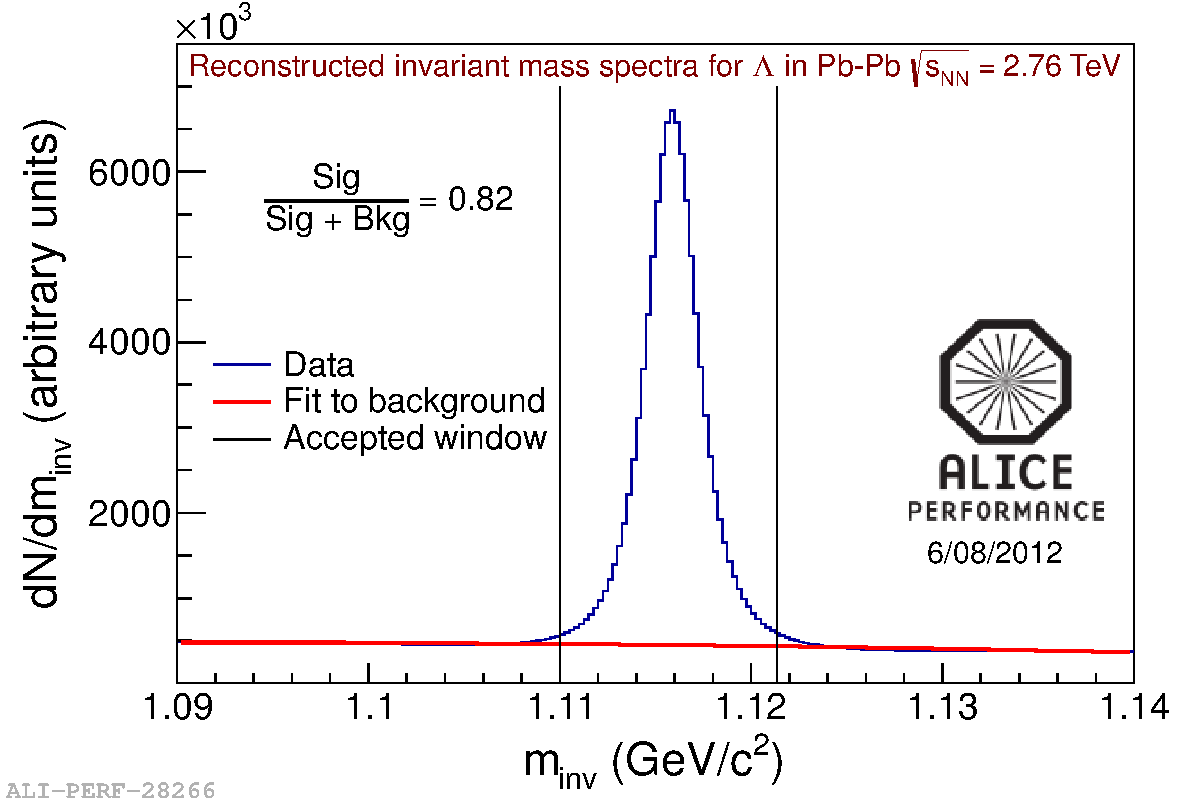
\includegraphics[scale=0.6]{2012-Aug-07-LamInvMass_Perf.pdf}
\caption[Invariant mass distribution for reconstructed $\Lambda$]{Invariant mass distribution for reconstructed $\Lambda$ using the main analysis cuts.  The red line shows a fourth order polynomial fit to the background, which is used to estimate the number of real and accidental $\Lambda$.  The estimated ratio of real $\Lambda$ to all reconstructed $\Lambda$ in the signal region ($ 1.11 < m_{\rm inv} < 1.12136$ GeV/${\rm c^2}$) shown in this plot is approximately 0.82.  Candidate for performance status.}
\label{fig:MassLooseCut}
\end{figure}

\begin{figure}[hbtp]
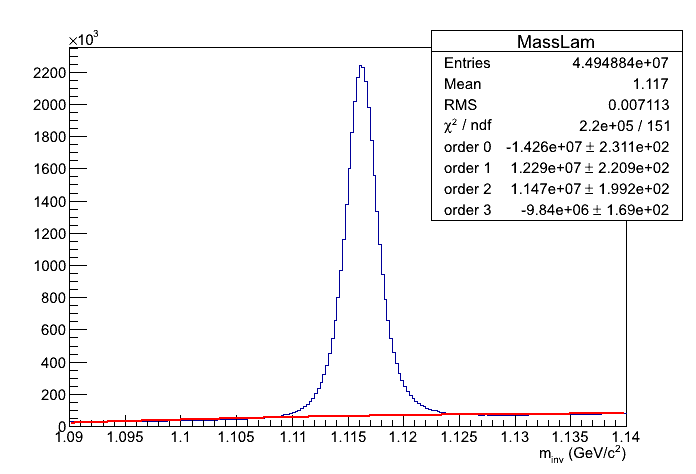
\includegraphics[scale=0.5]{11h_V0_MassLam_TightCuts.png}
\caption[Invariant mass distribution for reconstructed $\Lambda$ using tight cuts]{Invariant mass distribution for reconstructed $\Lambda$ using tight cuts.  Here, $sig/(sig+bkg) \approx 0.92$.}
\label{fig:MassTightCut}
\end{figure}

\begin{figure}[hbtp]
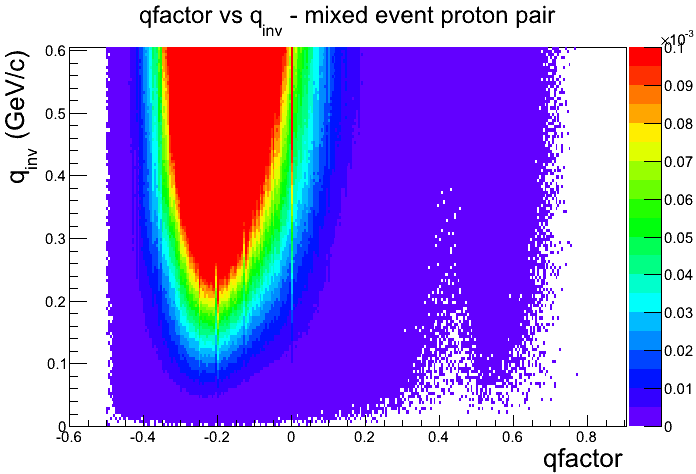
\includegraphics[scale=0.5]{Qfac_MixedEvent.png}
\caption[$qfactor$ vs $q_{inv}$ distribution of mixed-event pairs]{Scaled $qfactor$ vs $q_{inv}$ distribution of mixed-event proton-daughter pairs.  Since the daughters come from two different events, two-track reconstruction effects are absent.}
\label{fig:QfacMixed}
\end{figure}

\begin{figure}[hbtp]
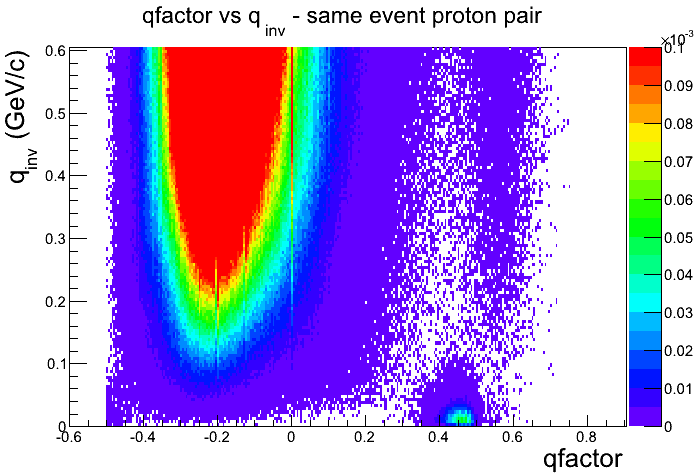
\includegraphics[scale=0.5]{Qfac_SameEvent.png}
\caption[$qfactor$ vs $q_{inv}$ distribution of same-event pairs]{Scaled $qfactor$ vs $q_{inv}$ distribution of same-event pairs.  Note the region of excess pairs (relative to Fig \ref{fig:QfacMixed}) at $qfactor \approx 0.45$ and $q_{inv} \leq 0.1$ GeV/c.  To excise splitting effects when constructing the correlation functions, V0 pairs are removed if their daughters have a $qfactor \geq 0.2$.}
\label{fig:QfacSame}
\end{figure}

\begin{figure}[hbtp]
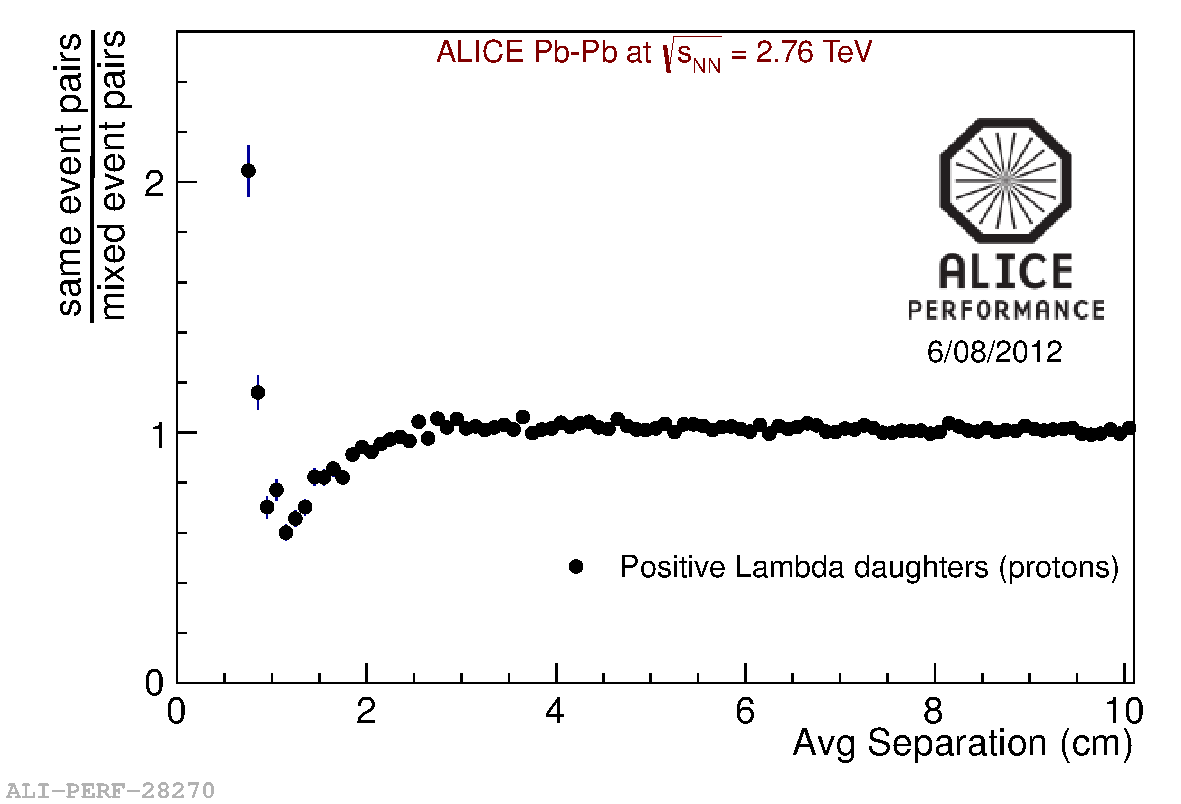
\includegraphics[scale=0.6]{2012-Aug-07-TwoTrack_Perf.pdf}
\caption[Correlation function showing two-track reconstruction effects]{Correlation function versus average separation distance in the TPC for proton daughters.  Constructed using same-event pairs over mixed-event pairs.  Both splitting (enhancement) and merging (suppression) effects are visible.  Candidate for performance status.}
\label{fig:Merging}
\end{figure}

\begin{figure}[hbtp]
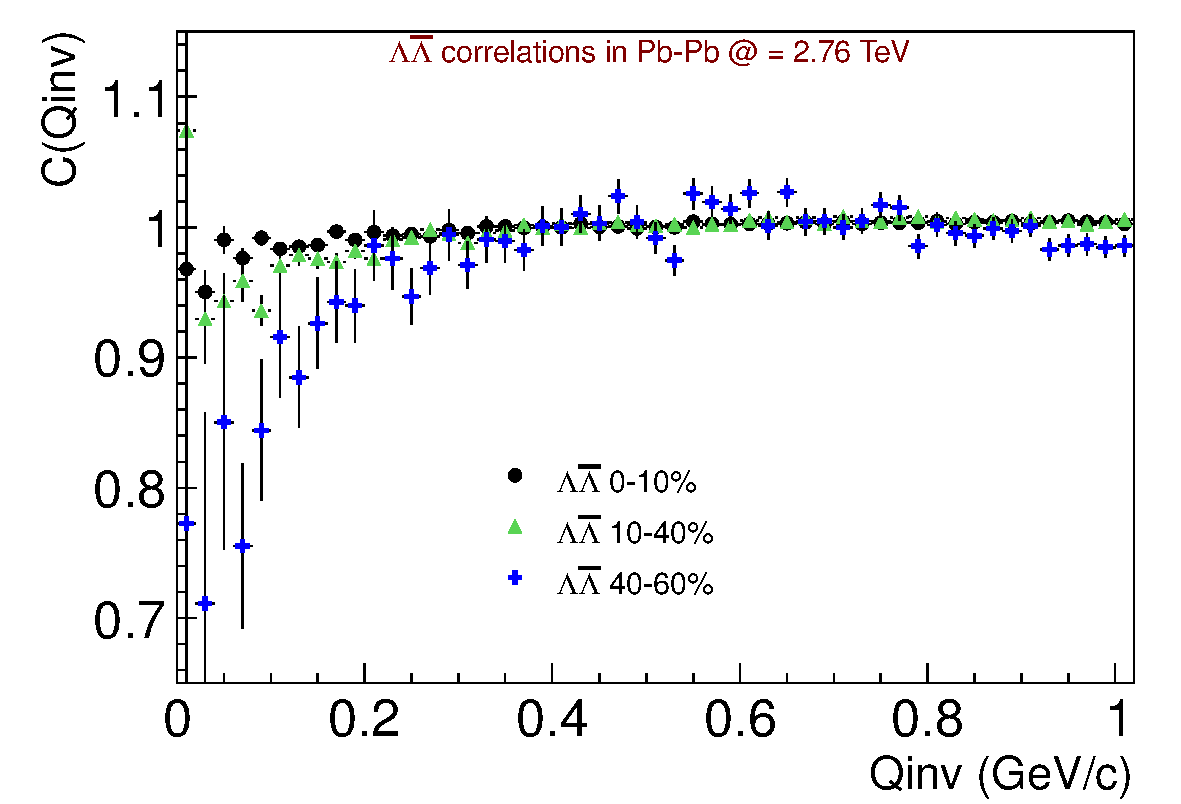
\includegraphics[scale=0.7]{LamALamCF_LooseCuts.pdf}
\caption[Correlation functions versus $q_{\rm inv}$ for $\Lambda\bar{\Lambda}$ pairs in three centrality ranges.]{Correlation functions versus $q_{\rm inv}$ for $\Lambda\bar{\Lambda}$ pairs.  Results are shown for the 0-10\%, 10-40\%, and 40-60\% centrality range.}
\label{fig:CFMixCentralities}
\end{figure}

\begin{figure}[hbtp]
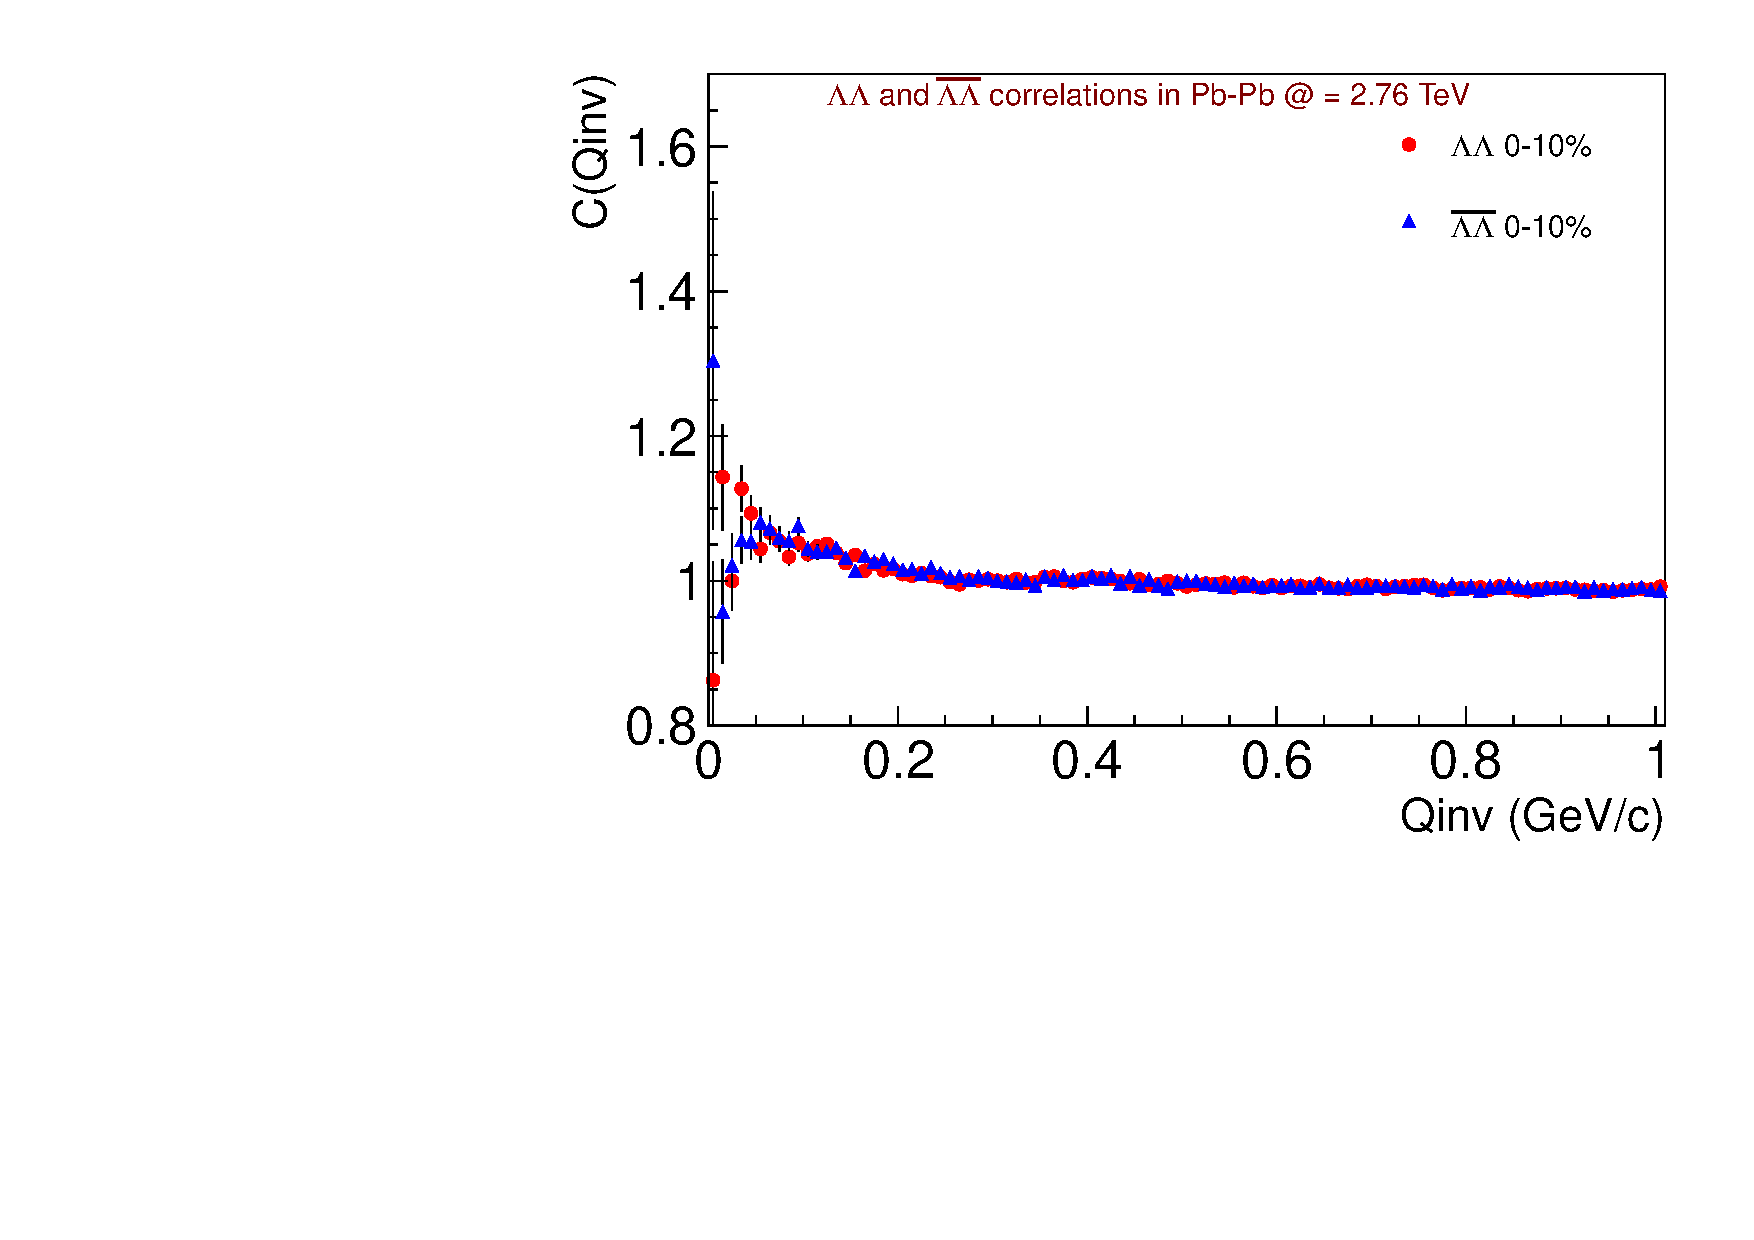
\includegraphics[scale=0.7]{CFs_main_note.pdf}
\caption[Correlation functions versus $q_{\rm inv}$ for $\Lambda\Lambda$ and $\bar{\Lambda}\bar{\Lambda}$ pairs.]{Correlation functions versus $q_{\rm inv}$ for $\Lambda\Lambda$ and $\bar{\Lambda}\bar{\Lambda}$ pairs.  Results are shown for the 0-10\% centrality range.}
\label{fig:CF}
\end{figure}

\begin{figure}[hbtp]
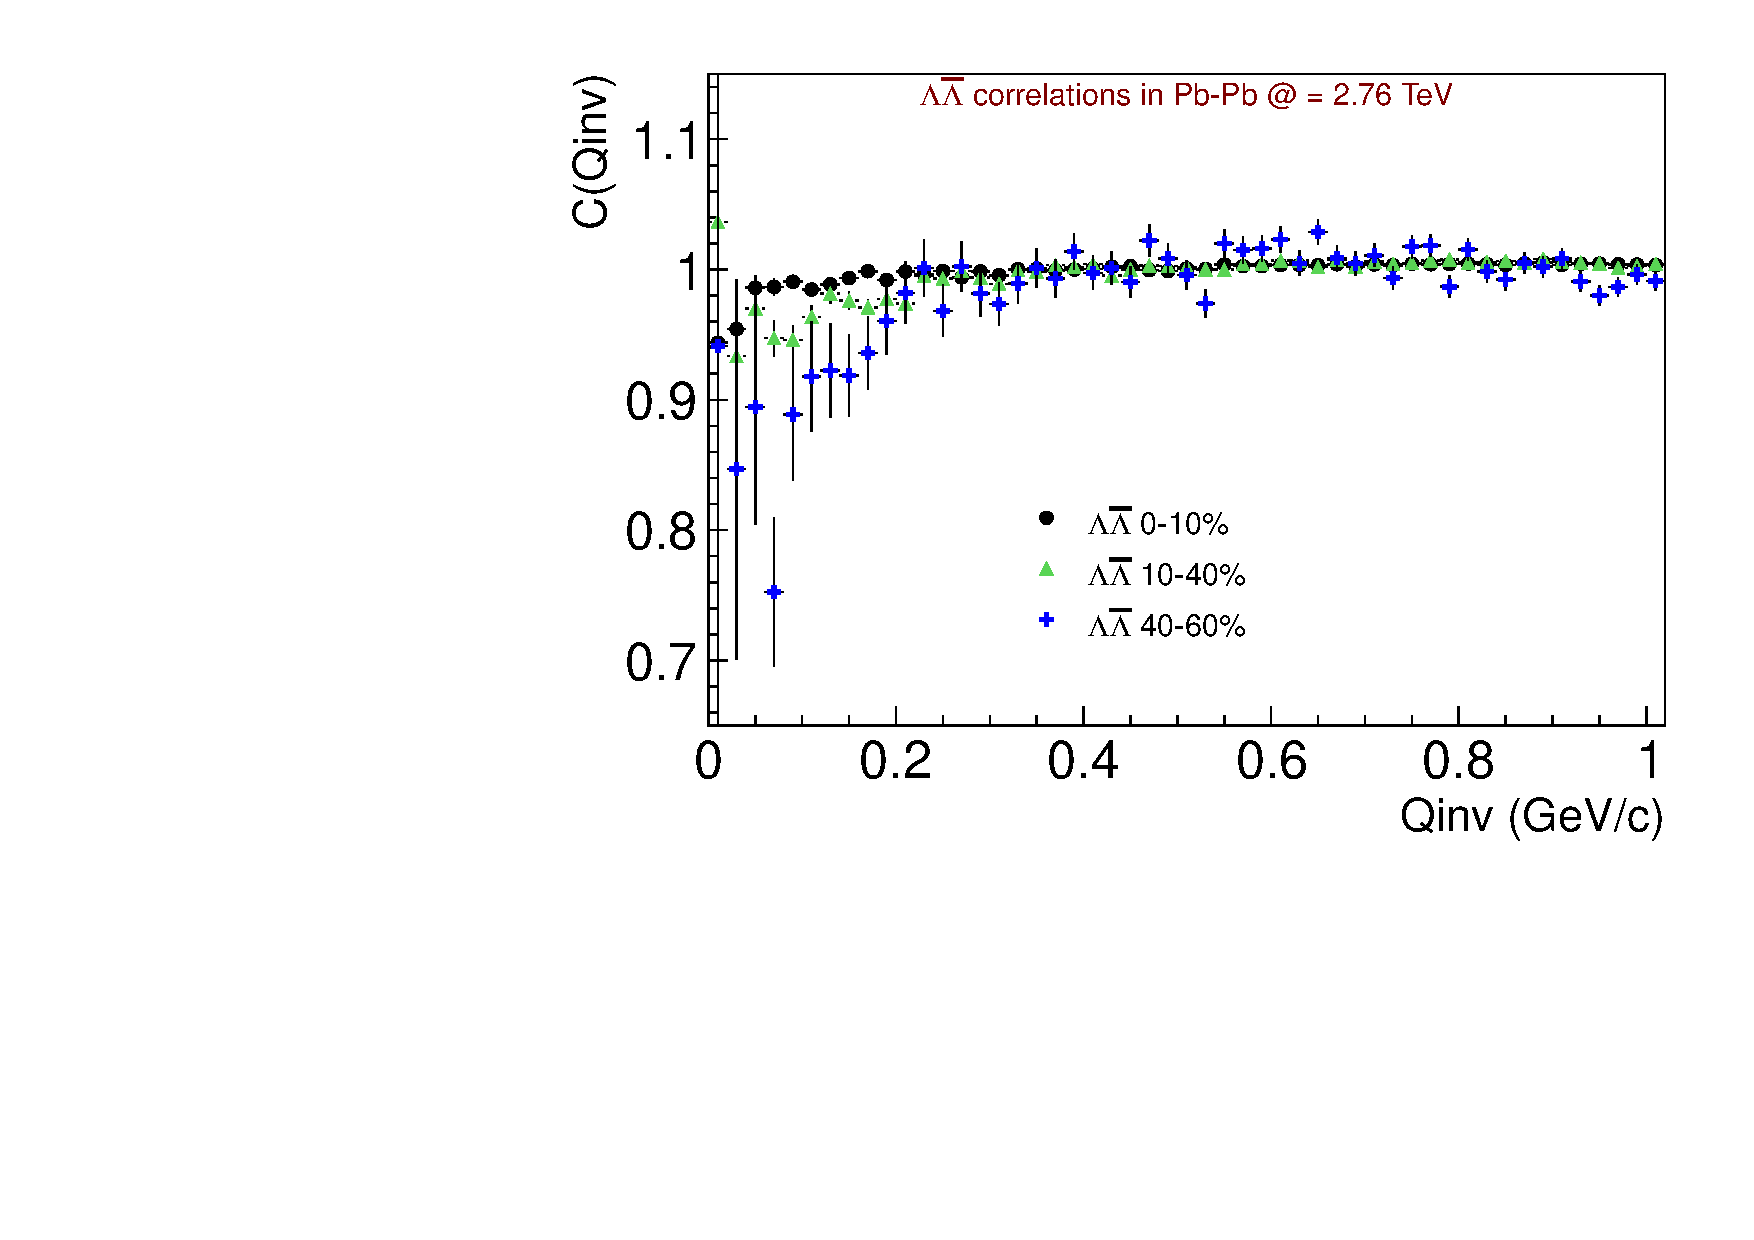
\includegraphics[scale=0.7]{MixCFs_No_MergeCut.pdf}
\caption[Correlation functions versus $q_{\rm inv}$ for $\Lambda\bar{\Lambda}$ pairs in three centrality ranges. No merging cuts]{Correlation functions versus $q_{\rm inv}$ for $\Lambda\bar{\Lambda}$ pairs (without cut on the average separation distance of the daughter pairs).  Results are shown for the 0-10\%, 10-40\%, and 40-60\% centrality range.}
\label{fig:CFNoMergeMix}
\end{figure}

\begin{figure}[hbtp]
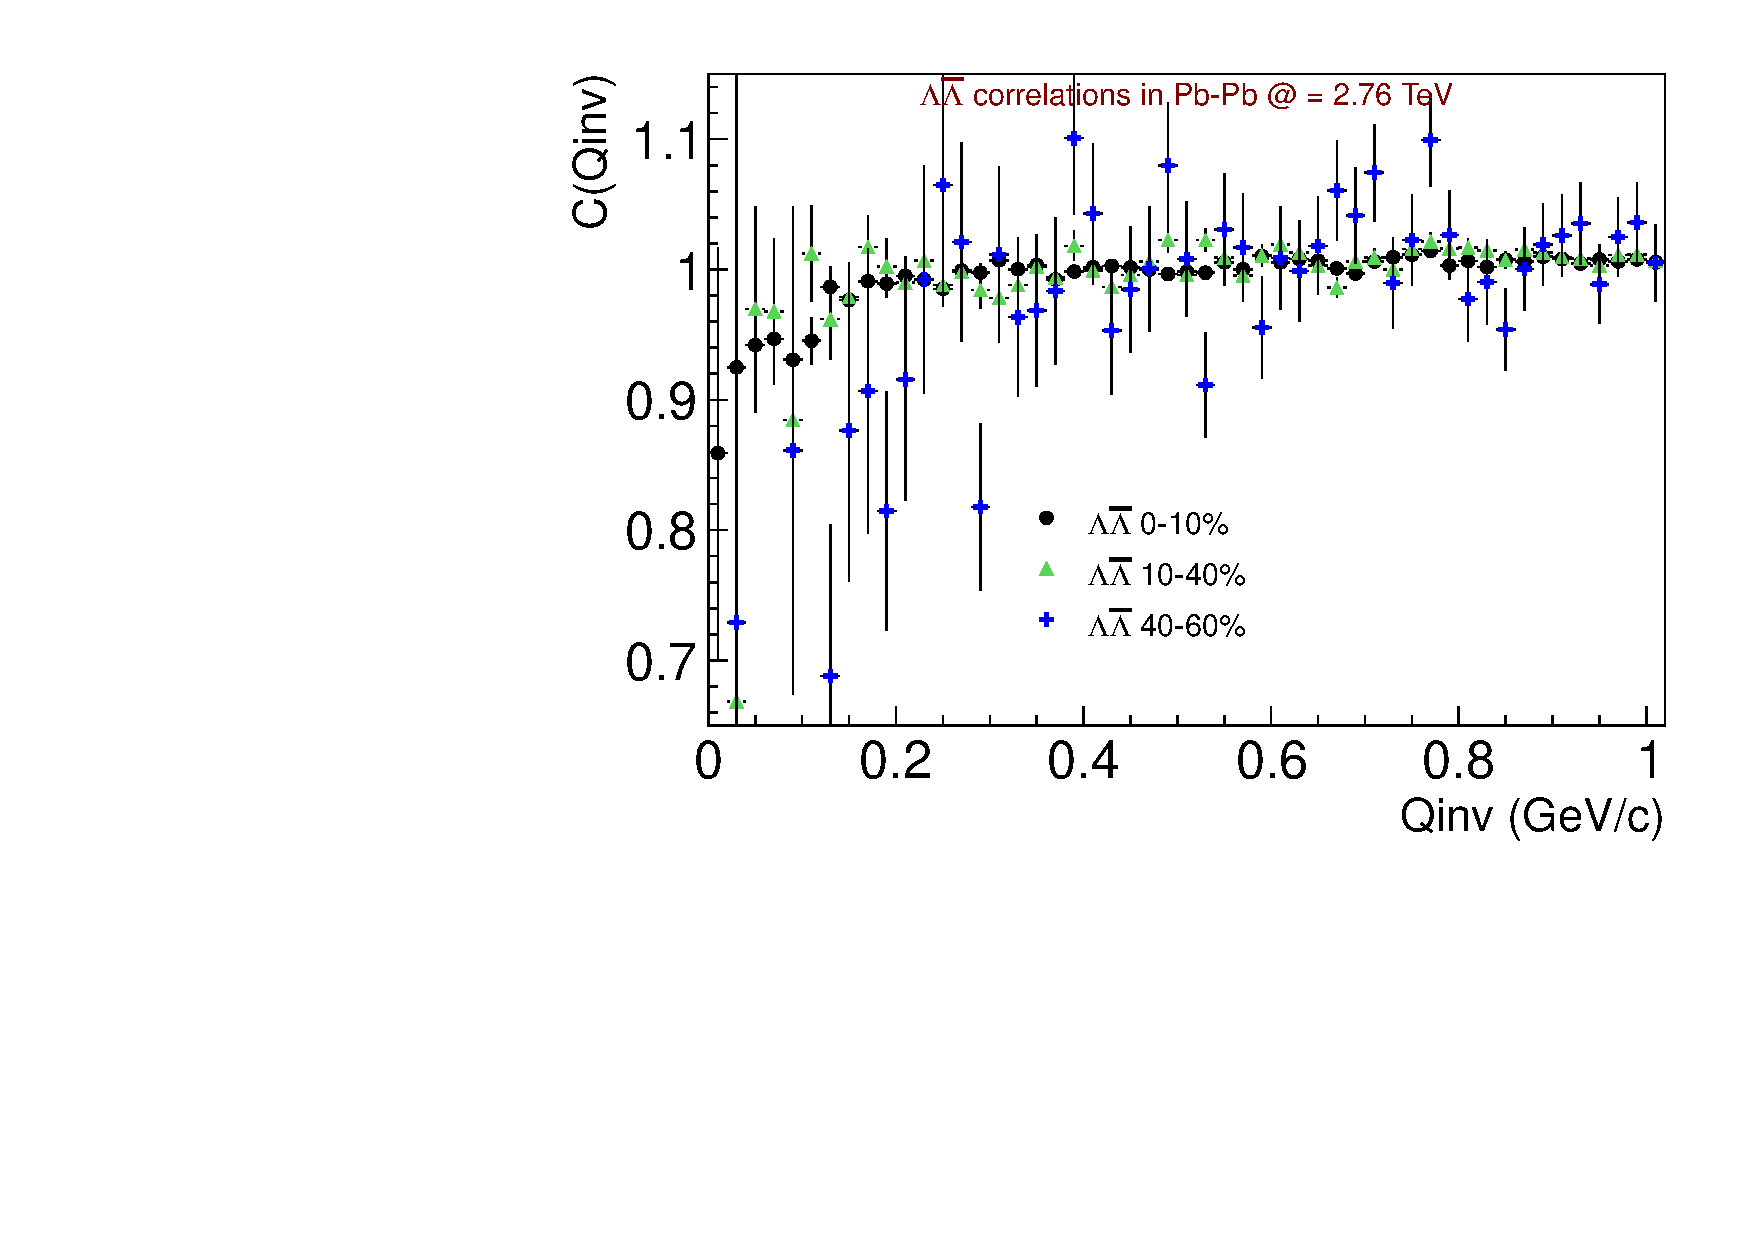
\includegraphics[scale=0.7]{Mix_Tight_cuts_ANote.pdf}
\caption{Correlation functions versus $q_{\rm inv}$ for $\Lambda\bar{\Lambda}$ pairs in three centrality ranges. Tight cuts.}
\label{fig:CFTightCutsMix}
\end{figure}

\begin{figure}[hbtp]
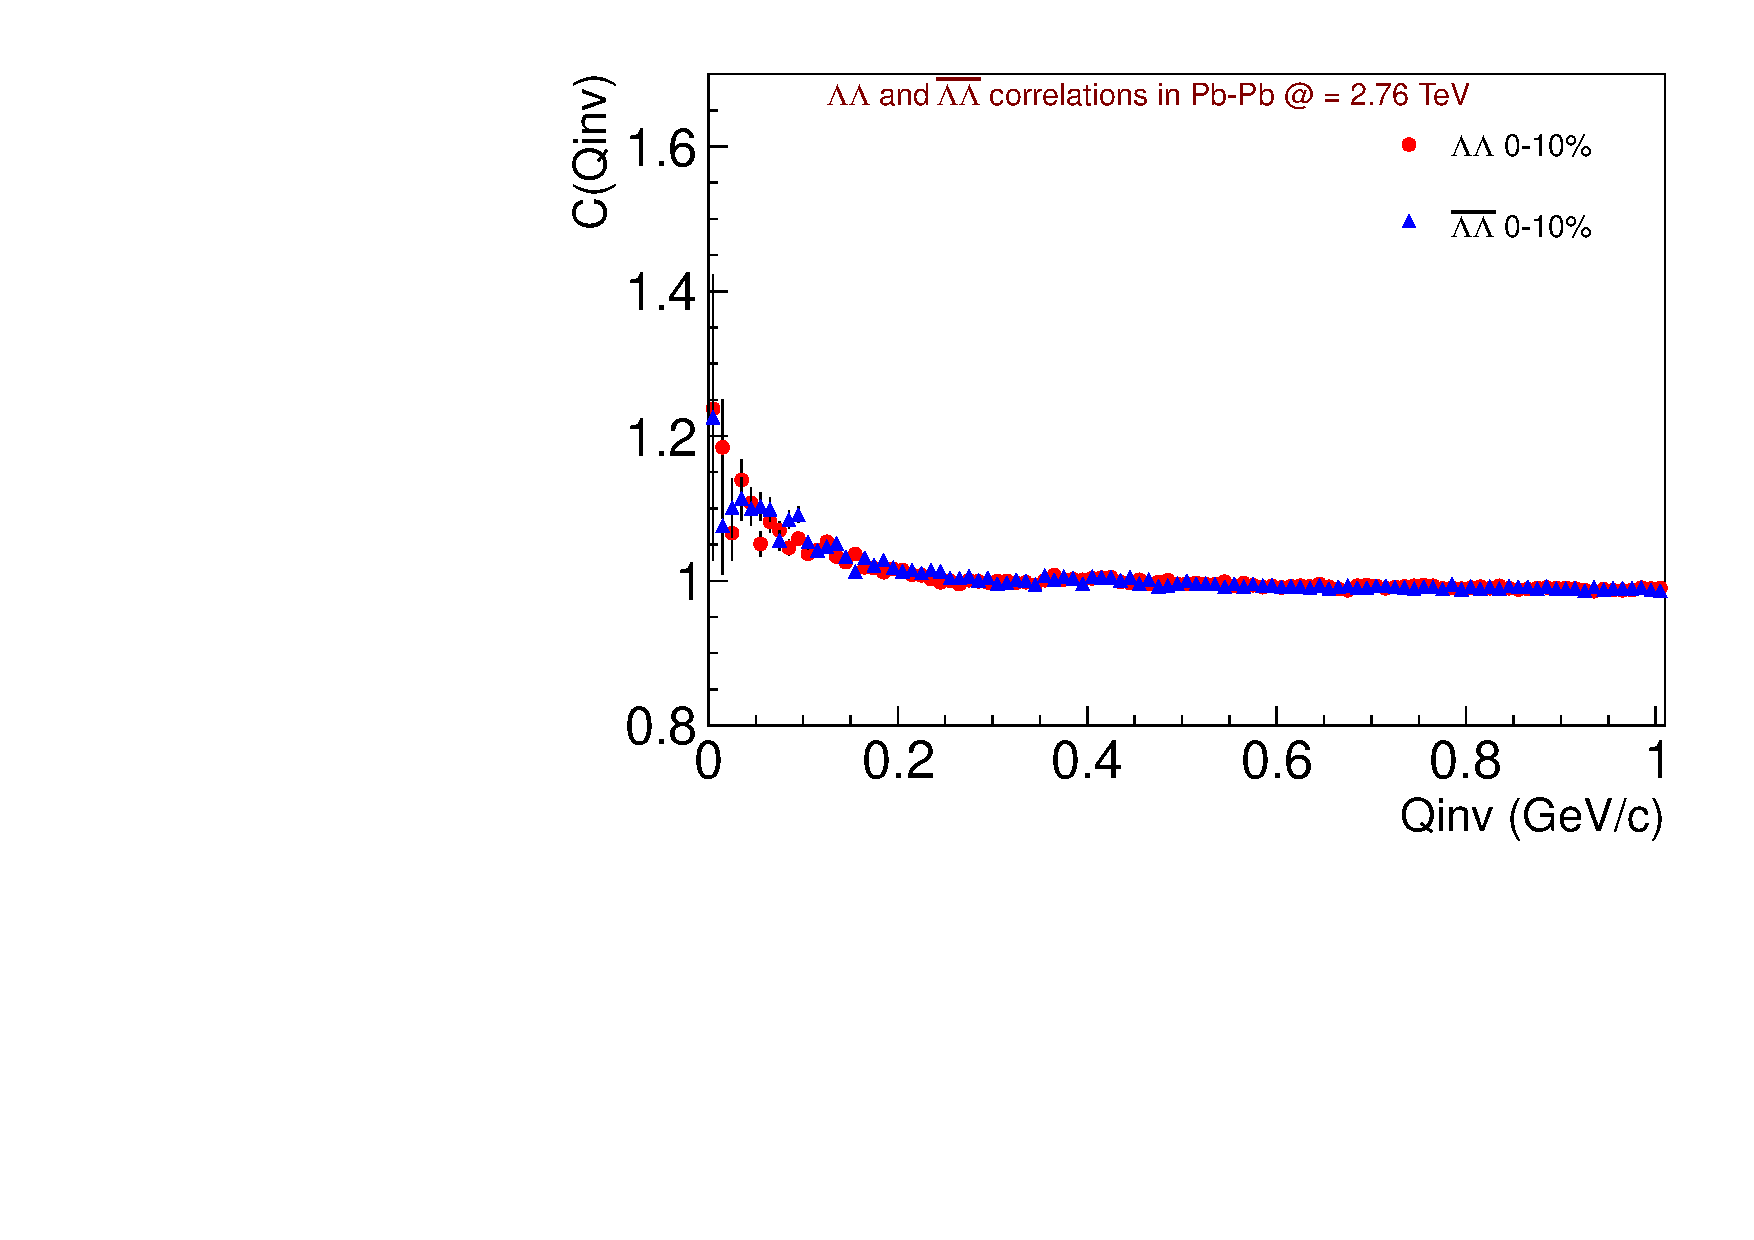
\includegraphics[scale=0.7]{CFs_noMergeCut_note.pdf}
\caption[Correlation functions versus $q_{\rm inv}$ for $\Lambda\Lambda$ and $\bar{\Lambda}\bar{\Lambda}$ pairs. No merging cuts]{Correlation functions versus $q_{\rm inv}$ for $\Lambda\Lambda$ and $\bar{\Lambda}\bar{\Lambda}$ pairs (without cut on the average separation distance of the daughter pairs).  Results are shown for the 0-10\% centrality range.}
\label{fig:CFNoMerge}
\end{figure}

\begin{figure}[hbtp]
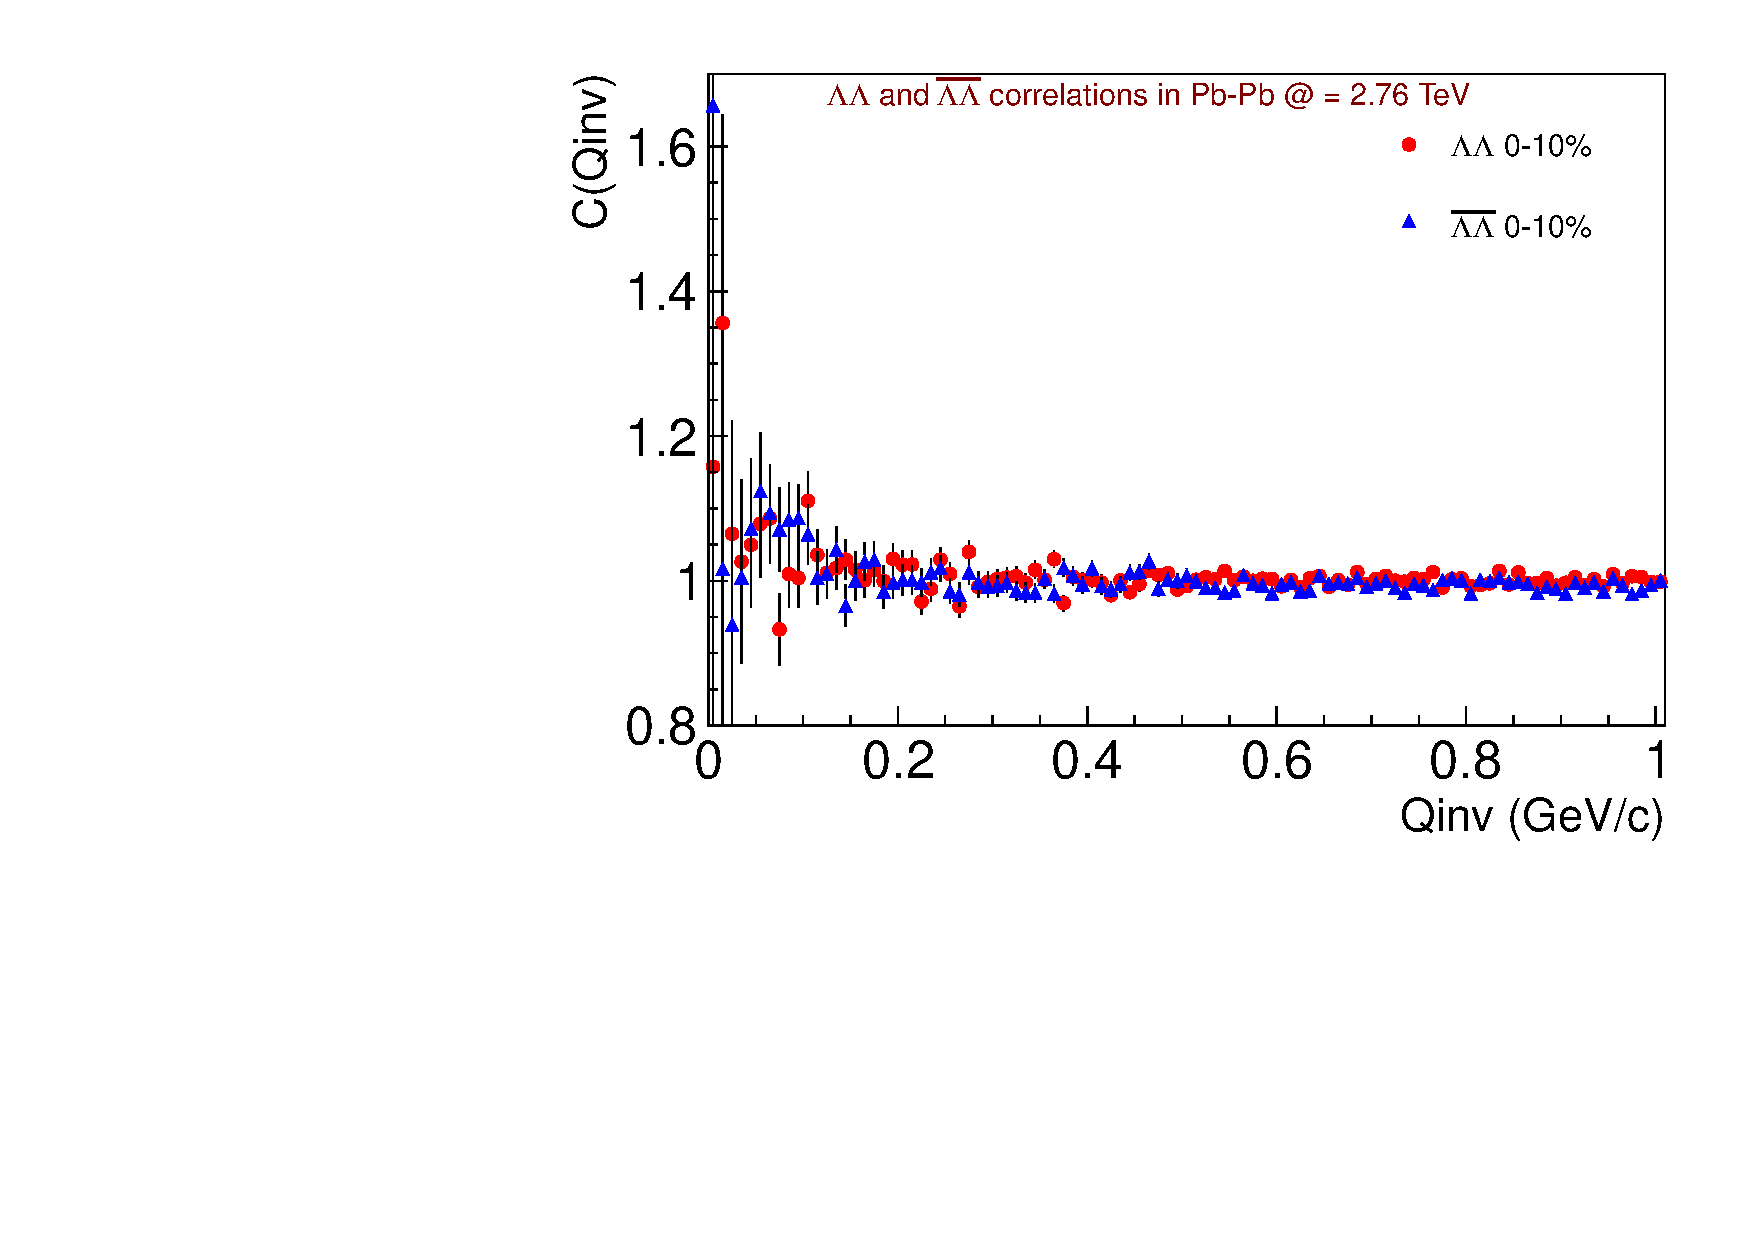
\includegraphics[scale=0.7]{CFs_tightcut_note.pdf}
\caption[Correlation functions versus $q_{\rm inv}$ for $\Lambda\Lambda$ and $\bar{\Lambda}\bar{\Lambda}$ pairs.  Tight cuts]{Correlation functions versus $q_{\rm inv}$ for $\Lambda\Lambda$ and $\bar{\Lambda}\bar{\Lambda}$ pairs using tight reconstruction cuts.  Results are shown for the 0-10\% centrality range.}
\label{fig:CFTightCuts}
\end{figure}

\begin{figure}[hbtp]
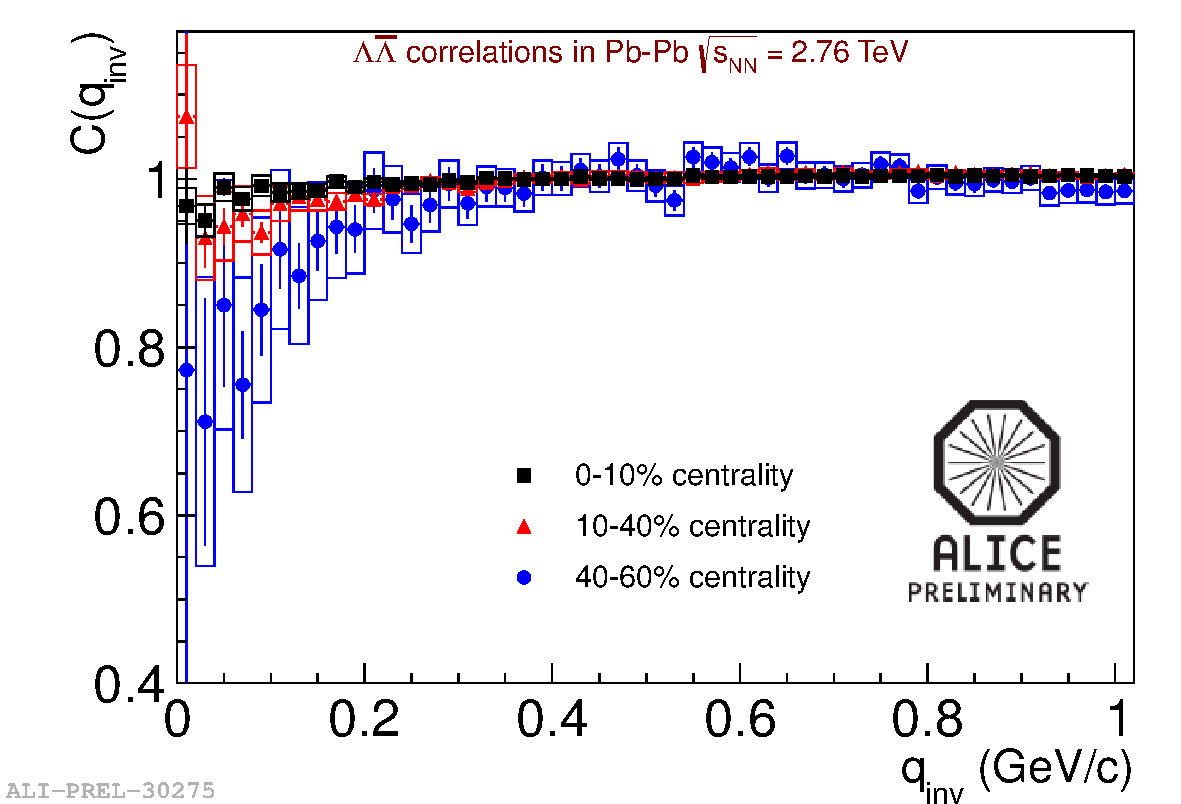
\includegraphics[scale=0.7]{2012-Jul-25-LamALamPrelim.pdf}
\caption[Correlation functions versus $q_{\rm inv}$ for $\Lambda\bar{\Lambda}$ pairs in three centrality ranges with systematic errors.]{Correlation functions versus $q_{\rm inv}$ with systematic errors for $\Lambda\bar{\Lambda}$ pairs. Systematics are computed by fitting the absolute value of the difference between Figure \ref{fig:CFMixCentralities} and Figure \ref{fig:CFTightCutsMix} with a 5th order polynormial. Results are shown for the 0-10\%, 10-40\%, and 40-60\% centrality range.}
\label{fig:CFMixSystematics}
\end{figure}

\bibliographystyle{plain}
\bibliography{bibfile}





%\end{document}               %%%%%%%%%%% put the body of the article here

\end{document}
